\documentclass{diploma}

\student{Концебалов Олег Сергеевич}
\group{М8О-409Б-22}
\theme{Автоматизированная платформа управления инфраструктурой с поддержкой подхода Architecture-as-Code}

\supervisor{Дзюба Дмитрий Владимирович}
\firstConsultant{Булакина Мария Борисовна}

\faculty{№ 8 <<Компьютерные науки и прикладная математика>>}
\department{806}
\speciality{01.03.02 <<Прикладная математика и информатика>>}
\profile{Информатика}

\departmentFullName{№ 806}
\headOfDepartment{Крылов Сергей Сергеевич}

% Дата. Оставляем пустое место для дня
\date{\uline{\hspace{24pt}} мая \the\year\ года}

\newacronym{api}{API}{Application Programming Interface, программный интерфейс взаимодействия компонентов системы}

\newacronym{http}{HTTP}{HyperText Transfer Protocol, прикладной протокол обмена данными между клиентом и сервером}

\newacronym{json}{JSON}{JavaScript Object Notation, текстовый формат представления структурированных данных}

\newacronym{dsl}{DSL}{Domain-Specific Language, предметно-ориентированный язык описания}

\newacronym{mvp}{MVP}{Minimum Viable Product, минимально жизнеспособная версия продукта}

\newacronym{sre}{SRE}{Site Reliability Engineering, инженерная практика обеспечения надёжности программных систем}

\newacronym{devops}{DevOps}{набор инженерных практик, объединяющих разработку, поставку и эксплуатацию программных систем}

\newacronym{vm}{VM}{Virtual Machine, виртуальная машина}

\newacronym{ssh}{SSH}{Secure Shell, протокол защищённого удалённого доступа к хосту}

\newacronym{fqdn}{FQDN}{Fully Qualified Domain Name, полное доменное имя хоста}

\newacronym{crd}{CRD}{Custom Resource Definition, механизм расширения Kubernetes API пользовательскими типами ресурсов}

\newacronym{sla}{SLA}{Service Level Agreement, формализованные требования к доступности и качеству сервиса}

\newacronym{onap}{ONAP}{Open Network Automation Platform, платформа автоматизации жизненного цикла сетевых сервисов}

\newglossaryentry{architectureascode}{
    name={Architecture-as-Code},
    description={подход к представлению архитектуры программной системы в машинно обрабатываемом виде, пригодном для версионирования, анализа и использования в автоматизированных процессах}
}

\newglossaryentry{infrastructureascode}{
    name={Infrastructure-as-Code},
    description={подход к описанию инфраструктурных ресурсов и конфигураций в виде кода или декларативных спецификаций, которые могут храниться в системе контроля версий; такие спецификации применяются автоматизированными инструментами}
}

\newglossaryentry{desiredstate}{
    name={Desired state},
    description={желаемое состояние инфраструктуры, описывающее, какие хосты и workload должны находиться под управлением платформы и какими свойствами они должны обладать}
}

\newglossaryentry{actualstate}{
    name={Actual state},
    description={фактическое состояние инфраструктуры, полученное из источников инвентаризации и наблюдения на момент проверки}
}

\newglossaryentry{drift}{
    name={Drift},
    description={расхождение между desired state и actual state}
}

\newglossaryentry{reconcile}{
    name={Reconcile},
    description={процесс приведения фактического состояния инфраструктуры к желаемому состоянию}
}

\newglossaryentry{controlloop}{
    name={Control loop},
    description={повторяемый цикл управления, включающий получение desired state, получение actual state, сравнение состояний, обнаружение drift и запуск reconcile-действий}
}

\newglossaryentry{inventory}{
    name={Inventory},
    description={представление сведений об управляемых хостах, их атрибутах, доступности источников данных и фактически наблюдаемых workload}
}

\newglossaryentry{workload}{
    name={Workload},
    description={программный компонент или служебный процесс, размещаемый на управляемом хосте}
}

\newglossaryentry{managedhost}{
    name={Managed host},
    description={хост, находящийся в зоне управления платформы и участвующий в цикле сопоставления desired state и actual state}
}

\newglossaryentry{sourceoftruth}{
    name={Source of truth},
    description={источник данных, рассматриваемый системой как авторитетный для определённого типа сведений}
}

\newglossaryentry{partialresult}{
    name={Partial result},
    description={частичный результат получения или обработки данных, при котором часть сведений недоступна}
}

\newglossaryentry{detector}{
    name={Detector},
    description={компонент логики DriftDetectorSvc, отвечающий за проверку конкретного workload и формирование результата обнаружения drift}
}

\newglossaryentry{operator}{
    name={Operator},
    description={компонент логики ReconcilerSvc, отвечающий за построение плана выполнения reconcile для конкретного поддерживаемого workload}
}

\newglossaryentry{executionplan}{
    name={Execution plan},
    description={структурированное описание действия reconcile, включающее выбранный playbook, целевой хост, компонент и параметры выполнения}
}

\newglossaryentry{snapshot}{
    name={Snapshot},
    description={согласованная копия состояния, хранящаяся сервисом в памяти и используемая для выдачи API-ответов без обращения к источникам данных при каждом запросе}
}

\newglossaryentry{structurizr}{
    name={Structurizr},
    description={инструмент и формат описания архитектуры программных систем, поддерживающий C4-модель и экспорт архитектурной модели в JSON-представление}
}

\newglossaryentry{cadvisor}{
    name={cAdvisor},
    description={инструмент сбора сведений о контейнерах и их состоянии, используемый в текущем MVP как источник actual state для контейнерных workload}
}

\newglossaryentry{ansiblerunner}{
    name={Ansible Runner},
    description={инструмент программного запуска Ansible playbook, используемый в ReconcilerSvc для выполнения reconcile-действий}
}

\newglossaryentry{parsersvc}{
    name={ParserSvc},
    description={сервис платформы, отвечающий за разбор Structurizr JSON, построение host-centric desired state и выдачу этого состояния через API}
}

\newglossaryentry{inventorysvc}{
    name={InventorySvc},
    description={сервис платформы, отвечающий за формирование actual state управляемых хостов на основе bootstrap-описания и данных внешних источников}
}

\newglossaryentry{driftdetectorsvc}{
    name={DriftDetectorSvc},
    description={сервис платформы, сравнивающий desired state и actual state, обнаруживающий drift и отправляющий reconcile-команды}
}

\newglossaryentry{reconcilersvc}{
    name={ReconcilerSvc},
    description={сервис платформы, принимающий reconcile-команды, выбирающий operator и асинхронно запускающий действия восстановления}
}


\addbibresource{main.bib}

\begin{document}
    \maketitle

    % \includepdf[pages=-]{extra/task} % Задание
    \setcounter{page}{2} % Устанавливает счётчик страниц

    \abstract % Структурный элемент: РЕФЕРАТ

\keywords{УПРАВЛЕНИЕ ИНФРАСТРУКТУРОЙ, ARCHITECTURE-AS-CODE, DESIRED STATE, ACTUAL STATE, DRIFT DETECTION, RECONCILE, CONTROL LOOP, INVENTORY, SRE, DEVOPS}

Выпускная квалификационная работа посвящена автоматизированному управлению инфраструктурой. Актуальность темы обусловлена необходимостью контроля соответствия между архитектурным описанием и фактическим состоянием без участия человека. В распределенных системах такая согласованность нарушается из-за ручных изменений, неполных процедур развертывания, сбоев и различий между средами. Возникающие расхождения рассматриваются как drift и требуют своевременного обнаружения и устранения.

Цель работы --- спроектировать и реализовать автоматизированную платформу управления инфраструктурой с поддержкой подхода Architecture-as-Code, обеспечивающую формирование desired state, получение actual state, обнаружение drift и инициирование reconcile для приведения инфраструктуры к заданному состоянию. Для этого выполнен анализ предметной области, проведено сравнение существующих решений, сформулированы требования к платформе, спроектирована архитектура и реализованы основные компоненты программного решения.

Практическим результатом работы стала MVP-реализация Infrastructure Management Platform, поддерживающая контроль наличия компонент \texttt{node\_exporter} и \texttt{cadvisor}. На данном сценарии подтверждена работоспособность полного цикла управления: архитектурное описание используется как источник desired state, inventory-слой формирует actual state, drift detection выявляет отсутствие требуемого компонента, а reconcile-контур инициирует его восстановление.

Предложенная платформа может рассматриваться как основа для дальнейшего развития внутреннего control plane, в котором Architecture-as-Code используется не только как способ документирования, но и как источник данных для автоматического управления инфраструктурой.
 % Реферат

    \tableofcontents % Содержание 
    \termsanddefenitions % Термины и определения
    \listofabbreviations % Перечень сокращений и обозначений
 
    \introduction % Структурный элемент: ВВЕДЕНИЕ

Современные программные системы всё чаще разворачиваются как совокупность сервисов, средств наблюдаемости и вспомогательных workload, распределённых между несколькими средами и управляемыми разными командами. В таких условиях инфраструктура перестаёт быть статическим набором серверов и конфигурационных файлов. Она становится изменяемой системой, состояние которой должно постоянно соответствовать архитектурным решениям и эксплуатационным требованиям.

Актуальность темы выпускной квалификационной работы обусловлена тем, что ручное сопровождение инфраструктуры плохо масштабируется при росте числа хостов и сервисов. Даже если исходная конфигурация была подготовлена корректно, со временем между проектным и фактическим состоянием возникают расхождения. Они появляются из-за ручных изменений, временной недоступности источников данных, отличий между окружениями и ошибок конфигурации. Такие расхождения принято рассматривать как drift: ситуация, при которой фактическое состояние инфраструктуры отличается от ожидаемого.

Проблема drift особенно существенна для эксплуатационных команд, поскольку она приводит к снижению предсказуемости системы. Инженер может считать, что на управляемом хосте должен быть запущен определённый workload, однако фактически он может отсутствовать, быть остановлен или не наблюдаться средствами инвентаризации. Без автоматизированного механизма сравнения целевого и фактического состояния такие проблемы обнаруживаются поздно: через инциденты, ручной аудит или косвенные симптомы в мониторинге.

Одним из способов снижения этих рисков является переход от разрозненных ручных операций к декларативной модели управления. В такой модели команда описывает желаемое состояние системы, а программный контур управления получает фактическое состояние, сравнивает его с желаемым и инициирует действия по устранению расхождений. Близкая идея лежит в основе Kubernetes-контроллеров: они наблюдают состояние объектов и выполняют действия, необходимые для приближения текущего состояния к заданному \cite{kubernetes_controllers}. Однако Kubernetes-ориентированные решения не всегда подходят для управления host-level workload вне кластера или для ситуаций, где источником целевого состояния является архитектурная модель системы.

В данной работе рассматривается подход Architecture-as-Code как способ превратить архитектурное описание в машинно обрабатываемый источник desired state. В отличие от обычной документации, которая часто используется только для коммуникации между участниками проекта, Architecture-as-Code позволяет хранить описание архитектуры в формальном виде, версионировать его и применять в автоматизированных процессах.

Целью выпускной квалификационной работы является разработка и обоснование архитектуры автоматизированной платформы управления инфраструктурой с поддержкой подхода Architecture-as-Code, обеспечивающей формирование desired state, получение actual state, обнаружение drift и инициирование reconcile для приведения инфраструктуры к целевому состоянию.

Для достижения поставленной цели необходимо решить следующие задачи:
\begin{enumerate}
    \item проанализировать проблему управления инфраструктурой в распределённых системах и определить роль drift detection в эксплуатационном контуре;
    \item обосновать применение Architecture-as-Code как источника desired state для платформы управления инфраструктурой;
    \item сформировать функциональные и нефункциональные требования к платформе;
    \item спроектировать архитектуру платформы и определить ответственность сервисов;
    \item реализовать компоненты платформы;
    \item провести проверку качества разработанного решения.
\end{enumerate}

Объектом исследования являются процессы управления инфраструктурой распределённых программных систем. Предметом исследования являются архитектурные и программные решения, обеспечивающие автоматизированное сопоставление desired state и actual state, обнаружение drift и выполнение reconcile-действий.

Методы исследования включают изучение предметной области, сравнительный анализ существующих инструментов, проектирование программной архитектуры, прототипирование, разработку микросервисных компонентов, модульное тестирование и экспериментальную оценку поведения системы.

Практическая значимость работы состоит в снижении объёма ручных операций при контроле состояния инфраструктуры и в повышении наблюдаемости расхождений между архитектурным описанием и фактическим состоянием управляемых хостов. Разработанная платформа может использоваться как основа для дальнейшего развития внутреннего control plane, в котором архитектурная модель становится не только документацией, но и источником данных для автоматизированного управления.

Структура работы соответствует логике исследования и разработки. В первой главе рассматриваются теоретические основы управления инфраструктурой, понятия desired state, actual state, drift и reconcile, а также анализируются существующие инструменты и подходы. Во второй главе выполняется проектирование автоматизированной платформы управления инфраструктурой. В третьей главе описывается реализация основных компонентов платформы. В четвёртой главе приводится исследование и оценка качества разработанного решения. В пятой главе рассматриваются практическая значимость, ограничения текущего MVP и направления дальнейшего развития. В заключении формулируются основные результаты работы.

    \section{ТЕОРЕТИЧЕСКИЕ ОСНОВЫ И АНАЛИТИЧЕСКИЙ ОБЗОР ПОДХОДОВ К УПРАВЛЕНИЮ ИНФРАСТРУКТУРОЙ}

Инфраструктура современной программной системы включает вычислительные узлы, сетевые настройки, контейнеры, системные сервисы, средства наблюдаемости и прикладные workload. При росте числа команд, окружений и управляемых хостов поддержание согласованного состояния перестает быть задачей разовой настройки и превращается в непрерывный эксплуатационный процесс.

В рамках данной работы инфраструктура рассматривается не только как набор ресурсов, которые необходимо создать, но и как изменяемая система, состояние которой должно постоянно сопоставляться с архитектурным описанием. Такой взгляд близок к модели управления Kubernetes: пользователь описывает желаемое состояние объектов, а контроллеры наблюдают фактическое состояние и выполняют действия для приближения системы к целевому виду \cite{kubernetes_controllers,kubernetes_objects}. Отличие рассматриваемой платформы состоит в том, что она ориентирована не на внутренние объекты Kubernetes-кластера, а на более общий контур управления архитектурных манифестов.

В данной главе рассматриваются ключевые понятия, необходимые для постановки задачи: desired state, actual state, drift, reconcile, Infrastructure-as-Code и Architecture-as-Code. Далее проводится анализ существующих решений и формулируются ограничения, которые мотивируют разработку собственной платформы.

\subsection{Проблема управления инфраструктурой в распределённых системах}

Распределенная система редко существует в единственном экземпляре. Как правило она разворачивается в нескольких средах: разработки, тестовой, preproduction и production. Каждая среда содержит собственный набор хостов, контейнеров, вспомогательных сервисов, источников телеметрии и конфигураций. Даже если первоначально такие среды настроены одинаково, со временем между ними возникают расхождения.

Причины расхождений разнообразны. Часть изменений вносится вручную в ходе оперативного устранения инцидентов. Часть появляется из-за неполных или устаревших инструкций развертывания. Часть связана с особенностями конкретного окружения: отличающимися версиями пакетов, сетевыми ограничениями, частично выполненными rollout-процедурами. В результате фактическое состояние инфраструктуры постепенно отходит от того состояния, которое команда считает правильным.

Для SRE- и DevOps-команд это приводит к росту операционных затрат. Чем больше инфраструктурных объектов находится в зоне ответственности команды, тем дороже становится ручная верификация. Инженеры вынуждены поддерживать инвентарные списки, сверять конфигурации, запускать отдельные playbook, анализировать журналы выполнения и самостоятельно решать, какие изменения допустимо применить. Такой подход может быть приемлемым для небольшого числа хостов, но плохо масштабируется при увеличении числа окружений и команд.

Отдельный риск связан с тем, что инфраструктурное состояние часто описано в разных местах. Архитектурная документация может существовать отдельно от inventory, inventory отдельно от конфигурационных playbook, а фактическая информация о запущенных workload извлекаться из средств мониторинга или вручную с хостов. Например, сведения о контейнерах могут поступать из cAdvisor, а сведения о хостах и их атрибутах --- из систем инвентаризации уровня NetBox \cite{cadvisor_docs,netbox_docs}. Пока эти источники не сведены в единый управляемый контур, команда не получает надежного ответа на вопрос: соответствует ли инфраструктура тому, что было спроектировано.

Следовательно, задача управления инфраструктурой в распределенных системах должна рассматриваться как задача непрерывного сопоставления архитектурного описания и фактического состояния. Для этого необходимы: формализованный источник целевого состояния, механизм получения актуального состояния, компонент сравнения, правила безопасной обработки неполных данных и механизм приведения системы к целевому виду.

\subsection{Desired state, actual state, drift и reconcile как базовая модель управления}

В основе автоматизированного управления инфраструктурой лежит различение желаемого и фактического состояния. Desired state описывает, каким должно быть состояние системы: какие хосты находятся под управлением, какие workload должны быть запущены, какие параметры необходимы для их развертывания, какие атрибуты характеризуют хосты и их назначение. Actual state, напротив, фиксирует состояние, наблюдаемое в текущий момент: какие хосты доступны, какие workload реально присутствуют, какие источники данных успешно отработали и где возникли ошибки.

Такое разделение позволяет перейти от императивной модели ``выполнить набор команд'' к декларативной модели ``поддерживать заданное состояние''. В императивной модели результат зависит от того, когда и как была выполнена команда. В декларативной модели главным артефактом становится целевое описание, а управляющая система должна регулярно проверять, достигнуто ли оно. Именно эта идея лежит в основе Kubernetes-контроллеров: контроллер наблюдает состояние ресурсов и выполняет действия, необходимые для приближения текущего состояния к желаемому \cite{kubernetes_controllers}.

Drift представляет собой обнаруженное расхождение между desired state и actual state. В простейшем случае drift означает, что компонент, обязательный в desired state, отсутствует в actual state. Более сложные виды drift могут включать несоответствие версии, конфигурации, режима запуска, сетевых параметров.

Reconcile обозначает процесс устранения drift, то есть выполнение действий, направленных на приведение фактического состояния к желаемому. Это управляемое действие, основанное на конкретном результате сравнения и ограниченное заранее определенным набором операторов. Такой подход снижает риск несанкционированных изменений: платформа не выполняет произвольный код, а выбирает один из поддержанных сценариев восстановления.

Для корректной реализации данной модели важна семантика неполных данных. Если источник actual state недоступен или вернул частичный результат, отсутствие информации не всегда можно трактовать как drift. Например, если система не смогла получить данные от источника наблюдения, она не должна автоматически устанавливать все отсутствующие в ответе компоненты. Без такого ограничения платформа может начать выполнять лишние reconcile-действия из-за сетевой ошибки или временной недоступности источника.

Поэтому безопасная control-loop модель должна различать три ситуации:
\begin{enumerate}
    \item компонент присутствует в desired state и подтвержденно отсутствует в actual state;
    \item компонент присутствует в desired state, но actual state неполон;
    \item desired state не требует компонента или компонент выключен.
\end{enumerate}

Только первая ситуация является основанием для reconcile. Вторая ситуация должна приводить к предупреждению, partial-статусу или пропуску части проверки. Третья не требует действий. Такая семантика особенно важна для инфраструктурной платформы, так как ошибочные автоматические изменения потенциально затрагивают рабочие хосты.

В результате desired state, actual state, drift и reconcile образуют базовую модель управления. Она позволяет описать инфраструктурный процесс как повторяемый цикл: получить целевое состояние, получить фактическое состояние, сравнить их, зафиксировать расхождения, выполнить допустимые действия восстановления и повторить проверку.

\subsection{Подходы Infrastructure-as-Code и Architecture-as-Code}

Infrastructure-as-Code является устоявшимся подходом, при котором инфраструктурные ресурсы описываются в машинно-читаемом виде. Такие описания могут храниться в системе контроля версий, проходить ревью и применяться автоматизированными инструментами. Преимущество Infrastructure-as-Code состоит в воспроизводимости: конфигурация инфраструктуры становится артефактом разработки, а не набором ручных действий конкретного инженера.

Классические инструменты Infrastructure-as-Code, такие как Terraform и Pulumi, ориентированы на описание ресурсов облаков, сетей, баз данных, Kubernetes-объектов и других инфраструктурных сущностей \cite{terraform_docs,pulumi_iac}. Их сильная сторона заключается в построении плана изменений, управлении зависимостями и повторяемом применении конфигурации.

Architecture-as-Code решает другую задачу. Если Infrastructure-as-Code описывает преимущественно инфраструктурные ресурсы и способы их создания, то Architecture-as-Code фиксирует архитектурное представление системы: компоненты, контейнеры, связи, deployment-узлы, среду размещения и дополнительные свойства.

Практическая ценность Architecture-as-Code проявляется в том, что архитектурная модель может стать источником desired state. Если deployment-описание содержит хосты, их атрибуты и размещенные на них workload, платформа может извлечь из него формализованное целевое состояние.

Для такого подхода подходит C4-модель, поскольку она задает несколько уровней описания программной системы: контекст, контейнеры, компоненты и код \cite{c4_model}. На уровне deployment-описания можно зафиксировать конкретные узлы и экземпляры контейнеров, то есть перейти от абстрактной архитектуры к инфраструктурно значимым данным. Structurizr DSL и экспортируемое JSON-представление дают техническую основу для такого машинного разбора \cite{structurizr_dsl}.

При этом Architecture-as-Code не заменяет Infrastructure-as-Code полностью. Эти подходы решают взаимодополняющие задачи. Infrastructure-as-Code отвечает за описание и создание ресурсов, а Architecture-as-Code позволяет связать архитектурное намерение с последующей проверкой фактической инфраструктуры.

\subsection{Анализ существующих решений}

Для обоснования необходимости собственной платформы был проведен анализ существующих решений. Сравнение выполнялось с точки зрения следующих критериев: наличие декларативного desired state, поддержка непрерывной реконсиляции, применимость вне Kubernetes, работа с host-level workload, сложность внедрения и соответствие идее Architecture-as-Code.

Ansible является одним из наиболее распространенных инструментов управления конфигурациями. Его важное преимущество заключается в agentless-подходе: для управления Linux-хостом обычно достаточно SSH-доступа. Это упрощает внедрение и снижает требования к целевым узлам.

Однако Ansible сам по себе не является непрерывным control plane. Playbook запускается как задача, выполняет набор операций и завершает работу. Если после этого на хосте произойдет drift, инструмент не обнаружит и не устранит его без внешней оркестрации. Кроме того, при росте числа хостов и групп inventory может стать сложным для сопровождения.

Terraform и Pulumi решают задачу декларативного описания инфраструктуры, но делают это преимущественно на уровне ресурсов и провайдеров. Они хорошо подходят для создания облачных объектов, сетей, managed-сервисов, Kubernetes-ресурсов и связанных зависимостей. Важное преимущество Terraform состоит в понятной модели plan/apply, а Pulumi --- в возможности использовать языки программирования для построения абстракций. Тем не менее оба подхода сохраняют характер запуска операции применения и не являются универсальным механизмом постоянного контроля host-level workload.

Kubernetes демонстрирует наиболее близкую к целевой платформе идею. В Kubernetes есть декларативные объекты, API-сервер, контроллеры и цикл согласования, который постоянно стремится привести observed state к desired state \cite{kubernetes_controllers,kubernetes_objects}. Операторы расширяют эту модель на доменные сущности \cite{kubernetes_operator_pattern}.

Ограничение Kubernetes-подхода состоит в его границах применимости. Если управляемая среда уже является Kubernetes-кластером, операторы и GitOps-инструменты дают сильный механизм реконсиляции. Но если необходимо управлять workload на VM, bare-metal-хостах или смешанной инфраструктуре, приходится либо переносить объекты в Kubernetes-модель, либо строить адаптеры.

Crossplane развивает идею Kubernetes как универсального control plane для внешних ресурсов. Через CRD и composition-механизм он позволяет описывать высокоуровневые инфраструктурные абстракции и управлять внешними объектами. Такой подход технологически мощен, но требует Kubernetes-кластера и компетенций в его расширении. Для задачи данной работы это важный ориентир, но не прямой заменитель: проектируемая платформа должна быть проще и фокусироваться на связке Architecture-as-Code, inventory, drift detection и reconcile.

Argo CD и Flux представляют GitOps-подход. Они автоматически синхронизируют Kubernetes-кластеры с конфигурациями, хранящимися в Git, и хорошо решают задачу drift для Kubernetes-ресурсов. Их ограничение связано с тем, что Git становится центральным runtime-источником изменений, а область управления остается в основном кластерной.

ONAP демонстрирует противоположный край спектра: это крупная платформа автоматизации жизненного цикла сетевых сервисов. Она содержит богатые подсистемы проектирования, inventory, политик, аналитики и closed-loop automation. В то же время ONAP ориентирована на телеком-домен и требует значительных ресурсов внедрения и эксплуатации. Для рассматриваемого проекта такой уровень комплексности является избыточным.

\begin{table}
    \centering
    \caption{Сравнение подходов и инструментов управления инфраструктурой}
    \label{tab:infra-tools-comparison}
    \footnotesize
    \begin{tabularx}{\textwidth}{|p{0.18\textwidth}|X|X|}\hline
    Инструмент & Сильные стороны & Ограничения относительно задачи работы \\ \hline
    Ansible & Agentless-модель, широкая экосистема модулей и ролей, удобство разового применения конфигураций по SSH \cite{ansible_docs}. & Job-based выполнение, отсутствие встроенной непрерывной реконсиляции, рост сложности inventory и playbook в крупных системах. \\ \hline
    Terraform & Декларативное описание ресурсов, план изменений, развитая экосистема провайдеров \cite{terraform_docs}. & Ориентация на provision инфраструктурных ресурсов и state-файл; host-level workload и непрерывная реконсиляция не являются основной моделью. \\ \hline
    Pulumi & Infrastructure-as-Code на языках программирования, возможность строить абстракции и тестировать код конфигурации \cite{pulumi_iac}. & Сохраняет job-based характер применения, требует навыков разработки и отдельного управления состоянием. \\ \hline
    Kubernetes Operators & Нативная control-loop модель, CRD и операторы для доменных объектов \cite{kubernetes_operator_pattern}. & Сильно привязаны к Kubernetes API и кластерной модели; bare-metal/VM-хосты и внешние workload требуют дополнительных адаптеров. \\ \hline
    Crossplane & Расширяет Kubernetes до control plane для внешних ресурсов, поддерживает композиции и непрерывное согласование \cite{crossplane_docs}. & Требует Kubernetes как базовую платформу, сложен для команд без Kubernetes-экспертизы, не фокусируется на host-level workload. \\ \hline
    Argo CD и Flux & GitOps-синхронизация Kubernetes-ресурсов, наблюдение drift в кластере, интеграция с Git \cite{argocd_docs,flux_docs}. & Ориентированы на Kubernetes-манифесты и Git как центральный источник; внешние хосты и архитектурные deployment-модели покрываются косвенно. \\ \hline
    ONAP & Комплексная автоматизация жизненного цикла сетевых сервисов, развитая модель inventory, политики и closed-loop automation \cite{onap_docs}. & Очень высокая сложность, телеком-ориентация, значительный операционный overhead для средних и небольших команд. \\ \hline
    \end{tabularx}
    \normalsize
\end{table}

Проведенный анализ показывает, что существующие инструменты закрывают отдельные части задачи, но не дают одновременно легковесной, domain-focused платформы, где Architecture-as-Code используется как источник desired state, inventory предоставляет actual state, отдельный сервис обнаруживает drift, а Reconciler выполняет набор действий восстановления.

\subsection{Ограничения существующих решений и мотивация собственной платформы}

Сравнение существующих решений позволяет выделить несколько повторяющихся ограничений. Первое ограничение связано с разрывом между архитектурным описанием и фактическим управлением инфраструктурой. Архитектура часто существует в виде диаграмм или текстовой документации, но эти артефакты не используются управляющими сервисами напрямую.

Второе ограничение состоит в job-based характере многих инструментов. Ansible, Terraform и Pulumi хорошо подходят для запуска конкретной операции, но для непрерывной реконсиляции требуется внешний цикл: расписание, pipeline, отдельный orchestrator или ручная инициатива инженера.

Третье ограничение относится к области применимости Kubernetes-ориентированных решений. Kubernetes Operators, Crossplane, Argo CD и Flux обладают сильной control-loop моделью, но их естественная среда --- Kubernetes API и Kubernetes-ресурсы. Для управления обычными хостами, Docker workload, агентами наблюдаемости или смешанной инфраструктурой их применение может оказаться слишком тяжелым.

Четвертое ограничение связано со сложностью крупных платформ. Системы уровня ONAP способны решать широкий набор задач автоматизации, но требуют значительного операционного overhead. Для команд, которым нужно решить конкретную проблему контроля drift и восстановления workload, внедрение такой платформы может быть несоразмерно сложным.

Мотивация собственной платформы заключается в поиске промежуточного решения. С одной стороны, оно должно использовать сильную идею Kubernetes-подобного control loop. С другой стороны, оно не должно требовать переноса всей инфраструктуры в Kubernetes или внедрения крупной enterprise-платформы. Такое решение должно быть понятным, расширяемым и пригодным для постепенного развития.

Для этого в проекте выбрана сервисная декомпозиция:
\begin{enumerate}
    \item ParserSvc отвечает за получение desired state из Architecture-as-Code-описания;
    \item InventorySvc отвечает за формирование actual state;
    \item DriftDetectorSvc сравнивает desired и actual state, обнаруживает drift и формирует reconcile-команды;
    \item ReconcilerSvc выполняет допустимые действия восстановления через операторную модель.
\end{enumerate}

Такое разделение позволяет независимо развивать источники desired state, источники actual state, набор detector-ов и набор reconcile-операторов. В MVP это выражено минимально: поддержаны Structurizr JSON как входной формат, cAdvisor\footnote{cAdvisor --- инструмент сбора и экспорта сведений о контейнерах и характеристиках их выполнения на хосте \cite{cadvisor_docs}.} как источник actual state и два workload-компонента: \texttt{node\_exporter} и \texttt{cadvisor}. Однако сама архитектура допускает расширение: добавление NetBox\footnote{NetBox --- система моделирования и документирования инфраструктуры, применяемая как source of truth для сетевых, серверных и связанных инфраструктурных ресурсов \cite{netbox_docs}.} как источника inventory, новых detector-ов, persistence-слоя, API истории drift и более сложных reconcile-сценариев.

Таким образом, разработка собственной платформы обоснована не отсутствием инструментов автоматизации как таковых, а отсутствием подходящего легковесного решения, объединяющего Architecture-as-Code, inventory, drift detection и reconcile в единую платформенную модель.

\subsection{Постановка задачи разработки платформы}

С прикладной точки зрения задача состоит в том, чтобы дать эксплуатационной команде инструмент регулярной проверки соответствия между архитектурным описанием и фактической средой исполнения. Такой инструмент должен помогать инженеру видеть, какие инфраструктурные workload ожидаются на управляемых хостах, какие из них реально наблюдаются, какие расхождения требуют внимания и какие восстановительные действия могут быть выполнены автоматически в пределах заранее заданных правил.

С учетом проведенного анализа задача выпускной квалификационной работы формулируется следующим образом: разработать и обосновать автоматизированную платформу управления инфраструктурой с поддержкой подхода Architecture-as-Code, которая извлекает desired state из архитектурного описания, получает actual state из источников inventory, обнаруживает drift между ними и инициирует reconcile для поддержанных workload.

Для достижения этой цели необходимо решить следующие инженерные задачи:
\begin{enumerate}
    \item определить модель desired state на основе Structurizr JSON и C4/deployment-представления;
    \item реализовать механизм получения actual state управляемых хостов;
    \item спроектировать сервис обнаружения drift с безопасной обработкой partial-данных;
    \item реализовать Reconciler с операторной моделью и асинхронным выполнением задач;
    \item определить API-контракты между сервисами;
    \item проверить работоспособность платформы тестами и экспериментальной оценкой ключевых сценариев.
\end{enumerate}

Таким образом, первая глава показывает, что рассматриваемая тема находится на пересечении Infrastructure-as-Code, Architecture-as-Code и control-loop автоматизации. Существующие решения дают важные ориентиры, прежде всего Kubernetes-модель controllers/reconcile, однако не закрывают в полной мере задачу легковесного управления host-level workload на основе архитектурного описания. Это обосновывает переход к проектированию собственной платформы, которому посвящена следующая глава.

    \section{ПРОЕКТИРОВАНИЕ АВТОМАТИЗИРОВАННОЙ ПЛАТФОРМЫ УПРАВЛЕНИЯ ИНФРАСТРУКТУРОЙ}

После анализа предметной области и существующих решений можно перейти к проектированию платформы. Основная проектная идея состоит в построении легковесного control plane, который использует Architecture-as-Code как источник desired state, получает actual state из inventory-источников, обнаруживает drift и инициирует ограниченные reconcile-действия.

\subsection{Функциональные и нефункциональные требования}

Требования к платформе формируются из целевого сценария: инженер описывает инфраструктурно значимую часть архитектуры, платформа строит desired state, получает actual state, сравнивает состояния и при необходимости инициирует reconcile. Такой сценарий требует как функциональных возможностей, так и эксплуатационных свойств, связанных с безопасностью автоматических действий.

К функциональным требованиям относятся:
\begin{enumerate}
    \item поддержка Architecture-as-Code-описания как источника desired state;
    \item построение host-centric desired state;
    \item получение actual state управляемых хостов через inventory-источники;
    \item хранение актуальных desired state и actual state в памяти сервисов;
    \item предоставление API для получения desired state и actual state;
    \item обнаружение drift между desired state и actual state;
    \item формирование reconcile-команд только для поддерживаемых workload;
    \item асинхронное принятие reconcile-команд и постановка задач на выполнение;
    \item фиксация partial result при неполных данных actual state.
\end{enumerate}

Нефункциональные требования отражают ограничения инфраструктурной автоматизации:
\begin{enumerate}
    \item модульность: компоненты desired state, actual state, drift detection и reconcile должны развиваться независимо;
    \item наблюдаемость: сервисы должны логировать ключевые стадии загрузки конфигурации, синхронизации, обнаружения drift и выполнения reconcile;
    \item безопасность автоматических действий: отсутствие данных не должно автоматически трактоваться как drift;
    \item расширяемость: должна существовать возможность добавления новых источников inventory, detector-ов и operator-ов;
    \item воспроизводимость конфигурации: параметры сервисов должны задаваться через внешние конфигурационные файлы;
    \item ограничение связности: сервисы должны взаимодействовать через явные HTTP-контракты;
    \item контейнеризуемость: каждый сервис должен поставляться как самостоятельный runtime-артефакт.
\end{enumerate}

\begin{table}
    \centering
    \caption{Связь требований с проектными решениями платформы}
    \label{tab:ch2-requirements-design}
    \footnotesize
    \begin{tabularx}{\textwidth}{|p{0.32\textwidth}|X|}\hline
    Требование & Проектное решение \\ \hline
    Использование Architecture-as-Code & Выделение ParserSvc, который читает Structurizr JSON и строит desired state \\ \hline
    Получение фактического состояния & Выделение InventorySvc, который формирует actual state на основе bootstrap-описания и данных cAdvisor \\ \hline
    Обнаружение drift & Выделение DriftDetectorSvc, сравнивающего desired state и actual state через HTTP API сервисов-источников \\ \hline
    Автоматическое восстановление & Выделение ReconcilerSvc, принимающего reconcile-команды и запускающего operator-specific execution plan \\ \hline
    Безопасная обработка неполных данных & Явная partial-семантика и запрет трактовать недоступность actual state как достаточное основание для произвольного reconcile \\ \hline
    Расширяемость & Registry-подход для detector-ов и operator-ов, конфигурируемые внешние источники, изоляция сервисов \\ \hline
    \end{tabularx}
    \normalsize
\end{table}

Таким образом, требования задают не только набор функций, но и архитектурные границы. Платформа должна быть достаточно автоматизированной, чтобы снижать ручную нагрузку, но достаточно ограниченной, чтобы автоматические действия оставались предсказуемыми.

\subsection{Общая архитектура платформы и внешние участники}

На уровне системного контекста платформа взаимодействует с несколькими внешними участниками и системами. Пользователь готовит Architecture-as-Code-описание инфраструктурно значимой части системы. В качестве такого описания используется Structurizr/C4-модель, из которой может быть получено JSON-представление для дальнейшего разбора \cite{c4_model,structurizr_dsl}.

Источниками actual state являются управляемые хосты и внешние системы инвентаризации. В текущем MVP фактические сведения о контейнерных workload извлекаются через cAdvisor. NetBox и другие источники сведений о хостах рассматриваются как направления расширения: архитектура предусматривает их наличие.

Системный контекст платформы представлен на рисунке~\ref{fig:ch2-system-context}.

\begin{figure}
  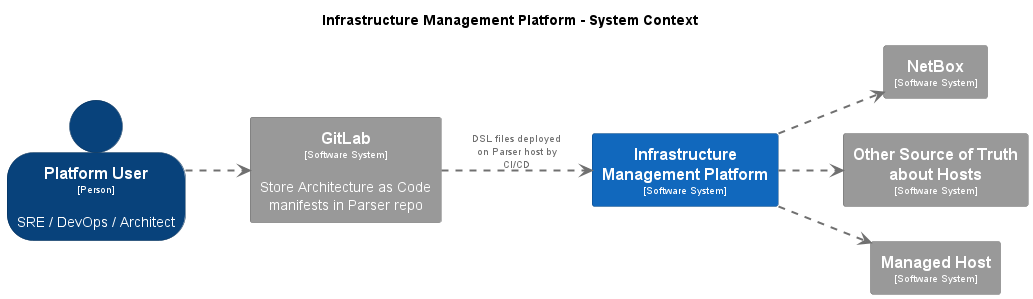
\includegraphics[width=0.95\linewidth]{../platform-arch-images/system-context.png}
  \caption{Системный контекст автоматизированной платформы управления инфраструктурой}
  \label{fig:ch2-system-context}
\end{figure}

Из рисунка~\ref{fig:ch2-system-context} видно, что платформа занимает промежуточное положение между архитектурным описанием и управляемой инфраструктурой. Она не заменяет репозиторий архитектурных артефактов и не является источником всех сведений о хостах. Ее роль состоит в связывании этих источников в один цикл управления: архитектурная модель задает целевое состояние, inventory-источники дают фактическое состояние, а reconcile-контур выполняет восстановление поддержанных workload.

\subsection{Контейнерная декомпозиция: ParserSvc, InventorySvc, DriftDetectorSvc, ReconcilerSvc}

Для реализации платформы выбрана сервисная декомпозиция. Каждый сервис отвечает за отдельную часть control loop и имеет собственный API. Такое разбиение уменьшает связность и позволяет независимо развивать источники desired state, источники actual state, алгоритмы detection и механизмы reconcile.

Контейнерная архитектура платформы представлена на рисунке~\ref{fig:ch2-container-diagram}.

\begin{figure}
  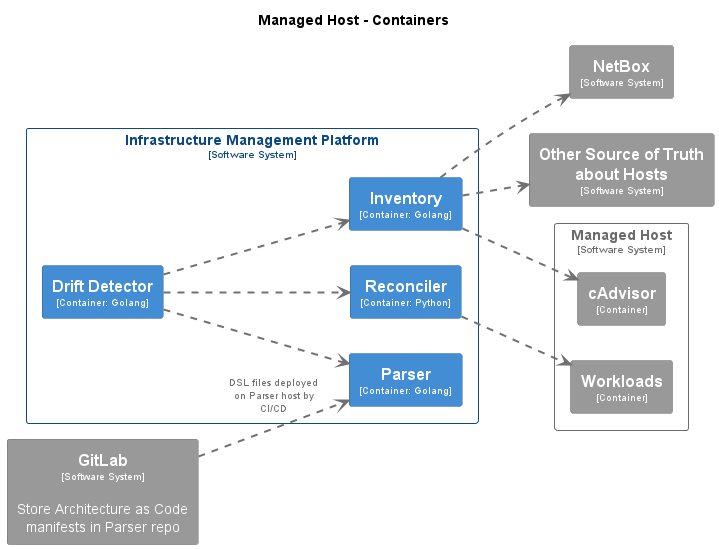
\includegraphics[width=0.95\linewidth]{../platform-arch-images/container-diagram.png}
  \caption{Контейнерная архитектура автоматизированной платформы управления инфраструктурой}
  \label{fig:ch2-container-diagram}
\end{figure}

ParserSvc отвечает за преобразование Architecture-as-Code-описания в desired state. Он выделяет deployment-узлы, свойства хостов и экземпляры контейнеров, после чего строит host-centric представление целевого состояния. ParserSvc предоставляет read-only API, через который другие сервисы могут получить полный desired state или сведения по отдельным хостам.

InventorySvc отвечает за actual state. Он загружает bootstrap-описание управляемых хостов, периодически обращается к источникам данных и формирует снимок фактического состояния. Сервис не проксирует внешний источник при каждом запросе, а обновляет внутренний snapshot и отдает его через read-only API. Такое решение снижает связанность API с доступностью внешнего источника в конкретный момент запроса.

DriftDetectorSvc является центральным компонентом цикла сравнения. Он получает desired state из ParserSvc и actual state из InventorySvc, сопоставляет хосты и применяет набор detector-ов для поддержанных workload. При обнаружении drift сервис формирует reconcile-команду и отправляет ее в ReconcilerSvc. Дополнительно DriftDetectorSvc отвечает за anti-spam/cooldown-семантику, чтобы повторяющийся drift не приводил к неограниченному числу одинаковых reconcile-запросов.

ReconcilerSvc принимает reconcile-команды и выполняет восстановление через operator-слой. Сервис реализован на Python/FastAPI и возвращает ответ \texttt{202 Accepted} после постановки задачи во внутреннюю очередь. Фактическое выполнение происходит асинхронно через Ansible Runner. Такое разделение важно, поскольку reconcile может занимать значительно больше времени, чем HTTP-запрос, и не должен блокировать DriftDetectorSvc до завершения playbook.

Контейнерная декомпозиция отражает естественное разделение данных:
\begin{enumerate}
    \item ParserSvc является источником desired state;
    \item InventorySvc является источником actual state;
    \item DriftDetectorSvc является сервисом принятия решения о drift;
    \item ReconcilerSvc является сервисом исполнения восстановительных действий.
\end{enumerate}

Такой подход также упрощает дальнейшее развитие. Например, добавление нового источника actual state требует изменения InventorySvc, но не должно менять ParserSvc. Добавление нового workload требует нового detector-а в DriftDetectorSvc и соответствующего operator-а в ReconcilerSvc, но не обязательно меняет API остальных сервисов.

\subsection{Модель desired state на основе Architecture-as-Code}

Desired state проектируется как host-centric модель. Это означает, что центральной сущностью становится хост, а требуемые workload рассматриваются как элементы, размещенные на этом хосте. Такой выбор соответствует задаче платформы: drift необходимо обнаруживать не в абстрактной архитектурной модели, а на конкретных управляемых хостах.

Входным форматом для ParserSvc является Structurizr JSON, для построения desired state используются его следующие части:
\begin{enumerate}
    \item \texttt{model.deploymentNodes} --- источник deployment-узлов, интерпретируемых как управляемые хосты;
    \item \texttt{model.softwareSystems[].containers} --- источник определений контейнеров и их имён;
    \item свойства deployment node --- источник \texttt{host\_id}, \texttt{fqdn}, \texttt{env}, \texttt{managed\_by}, \texttt{purpose} и дополнительных labels;
    \item свойства container instance --- источник признака включения workload, режима развертывания, image, version и port.
\end{enumerate}

Внутренняя модель desired state включает сущность \texttt{DesiredHost}. Для хоста обязательны \texttt{host\_id}, \texttt{fqdn}, \texttt{env}, \texttt{managed\_by}, \texttt{purpose}; поле \texttt{ip} является необязательным. Labels формируются из свойств deployment node и включают обязательные атрибуты окружения, владельца управления и назначения хоста. Такая модель позволяет в дальнейшем фильтровать хосты и группировать их по эксплуатационным признакам.

Workload в desired state описывается сущностью \texttt{DesiredWorkload}. Для MVP важны поля \texttt{name}, \texttt{enabled}, \texttt{deployment\_mode}, \texttt{image}, \texttt{version} и \texttt{port}. Поля \texttt{enabled} и \texttt{deployment\_mode} определяют, должен ли detector учитывать workload при проверке. Например, в текущей логике DriftDetectorSvc рассматривает workload только если он включен и имеет режим \texttt{container}.

С точки зрения проектирования важно, что ParserSvc не выполняет reconcile и не обращается к управляемым хостам. Его задача ограничена построением корректного snapshot desired state. Если часть манифестов некорректна, сервис должен зафиксировать ошибки, пропустить невалидные элементы и сохранить валидную часть состояния. Если ни один валидный JSON не загружен, сервис остается наблюдаемым через health endpoint, но readiness отражает отсутствие готового desired state.

Таким образом, модель desired state переводит Architecture-as-Code из уровня документации в уровень входных данных control loop. Это является ключевой особенностью платформы: архитектурная deployment-модель становится основанием для автоматизированной проверки инфраструктуры.

\subsection{Модель actual state и сбор данных через inventory}

Actual state проектируется как read-model текущего состояния управляемых хостов, он должен отражать наблюдаемое состояние инфраструктуры. Поэтому InventorySvc отделен от ParserSvc и имеет собственную модель данных, жизненный цикл синхронизации и partial-семантику.

Минимальный набор управляемых хостов задается через bootstrap-описание \texttt{selfProvisioning}. В нем указываются \texttt{id}, \texttt{fqdn} и labels хоста. Такой файл не является полноценным источником фактического состояния workload; он задает область наблюдения, то есть список хостов, по которым InventorySvc должен пытаться собрать данные.

Далее InventorySvc обращается к источникам actual state. Для каждого bootstrap-хоста сервис строит URL к cAdvisor endpoint, получает список контейнеров, нормализует ответ и преобразует его во внутреннюю модель \texttt{Workload}. Из ответа выделяются имя workload, image, runtime, источник данных и время наблюдения.

Для actual state проектируется явная модель статусов. Каждый хост может иметь статус \texttt{ok}, \texttt{partial}, \texttt{error} или \texttt{bootstrap\_only}. Дополнительно хранится \texttt{sourceStatus}: карта статусов по каждому источнику данных. Такой подход позволяет DriftDetectorSvc отличать подтвержденное отсутствие workload от отсутствия достоверных данных.

Partial result является отдельным проектным требованием. Если часть хостов или источников недоступна, InventorySvc не должен завершать работу ошибкой и не должен скрывать неполноту. Вместо этого он возвращает данные по доступным хостам и явно выставляет признаки \texttt{metadata.isPartial}, \texttt{failedHosts}, а также статусы по отдельным источникам. Такая модель повышает устойчивость платформы и снижает риск ошибочных reconcile-действий.

InventorySvc хранит actual state как in-memory snapshot. API читает уже подготовленный snapshot, а не инициирует сбор данных при каждом запросе. Это решение важно по двум причинам. Во-первых, оно отделяет частоту внешней синхронизации от частоты запросов других сервисов. Во-вторых, оно делает API-ответ согласованным: DriftDetectorSvc получает снимок состояния, сформированный в рамках завершенного цикла синхронизации.

\subsection{Сценарий drift detection и reconcile}

Основной сценарий платформы представляет собой последовательный цикл обработки. DriftDetectorSvc получает desired state от ParserSvc и actual state от InventorySvc. Далее он сопоставляет хосты, применяет detector-ы и при необходимости отправляет reconcile-команды в ReconcilerSvc.

Сопоставление хостов выполняется по \texttt{host\_id}; если оно не дает результата, используется fallback по \texttt{fqdn}. Такое решение повышает устойчивость к неполному заполнению данных, но сохраняет приоритет стабильного идентификатора. Если actual-host для desired-host не найден, ситуация фиксируется как partial, а хост пропускается. Это важно: отсутствие хоста в actual state не рассматривается как достаточное основание для автоматического восстановления всех его workload.

Detector-слой проектируется как расширяемый registry. Каждый detector отвечает за один поддерживаемый компонент и знает:
\begin{enumerate}
    \item как найти соответствующий workload в desired state;
    \item какие условия делают проверку применимой;
    \item как оценить полноту actual data;
    \item как определить drift;
    \item как сформировать reconcile-команду.
\end{enumerate}

В MVP поддержаны \texttt{node\_exporter} и \texttt{cadvisor}. Для \texttt{node\_exporter} drift означает, что workload включен в desired state, имеет режим \texttt{container}, но отсутствует в actual state при здоровом источнике cAdvisor. Для \texttt{cadvisor} дополнительно предусмотрен bootstrap-сценарий: если источник cAdvisor недоступен, сервис может инициировать установку cAdvisor, поскольку сам cAdvisor является необходимым компонентом для последующего получения actual state.

Перед отправкой reconcile-команды применяется anti-spam/cooldown-механизм. Его задача --- предотвратить повторную отправку одинаковых команд в коротком временном окне. Ключ cooldown строится по компоненту и FQDN хоста. Если для этой пары недавно уже отправлялся reconcile, повторная команда подавляется, а факт подавления фиксируется в статистике цикла.

ReconcilerSvc проектируется как асинхронный исполнитель. HTTP-запрос \texttt{POST /api/v1/reconcile} возвращает \texttt{202 Accepted}, если команда валидна и поставлена в очередь. Такой ответ означает принятие задачи, но не гарантирует успешное завершение действия на хосте. Это осознанная семантика MVP: результат выполнения фиксируется в логах, а повторная попытка может быть инициирована следующим циклом detection, если drift сохранится.

Operator-слой ReconcilerSvc отделяет API от конкретных playbook. Operator выбирает playbook и формирует execution plan, а Ansible Runner выполняет этот план на целевом хосте \cite{ansible_docs}. Такой подход сохраняет расширяемость: для нового workload необходимо добавить operator и playbook, не меняя общий API reconcile.

Сценарий drift detection и reconcile проектируется как безопасный и ограниченный. Платформа не пытается автоматически исправлять все возможные расхождения инфраструктуры. Она обнаруживает только поддержанные типы drift и выполняет только заранее определенные действия. Это соответствует природе MVP и снижает риск непредсказуемых изменений.

\subsection{Выбор технологий и границы MVP}

Технологический стек выбран исходя из задач отдельных сервисов. ParserSvc, InventorySvc и DriftDetectorSvc реализуются на Go. Этот выбор оправдан для сервисов, которым нужны компактные бинарные артефакты, простая контейнеризация, эффективная работа с HTTP API и конкурентными операциями.

ReconcilerSvc реализуется на Python/FastAPI. Этот выбор связан с естественной интеграцией Python-экосистемы с Ansible Runner. FastAPI предоставляет удобный способ описания HTTP API и валидации запросов через Pydantic, а Python позволяет напрямую использовать ansible-runner без дополнительного межъязыкового слоя.

В качестве формата Architecture-as-Code используется Structurizr JSON. Это решение связано с поддержкой C4-модели и возможностью описывать deployment-узлы и экземпляры контейнеров \cite{c4_model,structurizr_dsl}. Сервис ParserSvc читает именно JSON-представление, что уменьшает сложность реализации и делает входной контракт более явным.

cAdvisor выбран как минимальный источник actual state для контейнерных workload. Он предоставляет сведения о контейнерах на хосте, которые можно нормализовать до модели workload.

Ansible Runner выбран как механизм выполнения reconcile. Ansible хорошо подходит для agentless-доступа к хостам по SSH и для описания идемпотентных ролей установки контейнерных workload \cite{ansible_docs}. При этом сама платформа не становится ``оберткой над Ansible'': Ansible используется только внутри ReconcilerSvc как executor, а решение о drift принимается отдельным сервисом.

Границы MVP зафиксированы следующим образом:
\begin{enumerate}
    \item источник desired state --- Structurizr JSON;
    \item DSL-разбор внутри ParserSvc не выполняется;
    \item состояние сервисов хранится в памяти, persistence и история snapshot не реализованы;
    \item основной источник actual state --- cAdvisor;
    \item NetBox и другие источники рассматриваются как точки расширения;
    \item поддержанные workload --- \texttt{node\_exporter} и \texttt{cadvisor};
    \item drift-модель ограничена отсутствием требуемого контейнерного workload;
    \item результат reconcile не хранится как job history и не доступен через отдельный status API;
    \item безопасность API и аутентификация внешних вызовов находятся вне текущего MVP.
\end{enumerate}

Такие ограничения не противоречат цели работы. Напротив, они позволяют проверить основную архитектурную гипотезу: Architecture-as-Code может быть использован как источник desired state для автоматизированного управления инфраструктурой, если дополнить его inventory-слоем, drift detection и ограниченным reconcile-контуром.

Таким образом, в главе спроектирована автоматизированная платформа управления инфраструктурой с поддержкой подхода Architecture-as-Code. Определены требования, внешние участники, сервисная декомпозиция, модели desired state и actual state, сценарий drift detection/reconcile, технологический стек и границы MVP. Следующая глава посвящена реализации этих проектных решений в конкретных компонентах платформы.

    \section{РЕАЛИЗАЦИЯ КОМПОНЕНТОВ ПЛАТФОРМЫ}

После проектирования архитектуры следующим этапом стала реализация компонентов платформы. В соответствии с выбранной декомпозицией кодовая база разделена на четыре сервиса: \texttt{ParserSvc}, \texttt{InventorySvc}, \texttt{DriftDetectorSvc} и \texttt{ReconcilerSvc}. Каждый сервис реализует отдельную часть control loop и взаимодействует с остальными через HTTP API.

Реализация следует принципу разделения ответственности. Сервис разбора архитектурных манифестов не обращается к управляемым хостам, inventory-сервис не принимает решений о drift, сервис обнаружения drift не выполняет Ansible playbook, а reconciler не занимается построением desired state. Благодаря этому каждый компонент можно тестировать, развивать и расширять независимо.

\subsection{Реализация ParserSvc: загрузка Structurizr JSON, построение desired state, API}

\texttt{ParserSvc} реализован на Go и отвечает за преобразование Architecture-as-Code-описания в host-centric desired state. Компонентная структура сервиса представлена на рисунке~\ref{fig:ch3-parser-components}.

\begin{figure}
  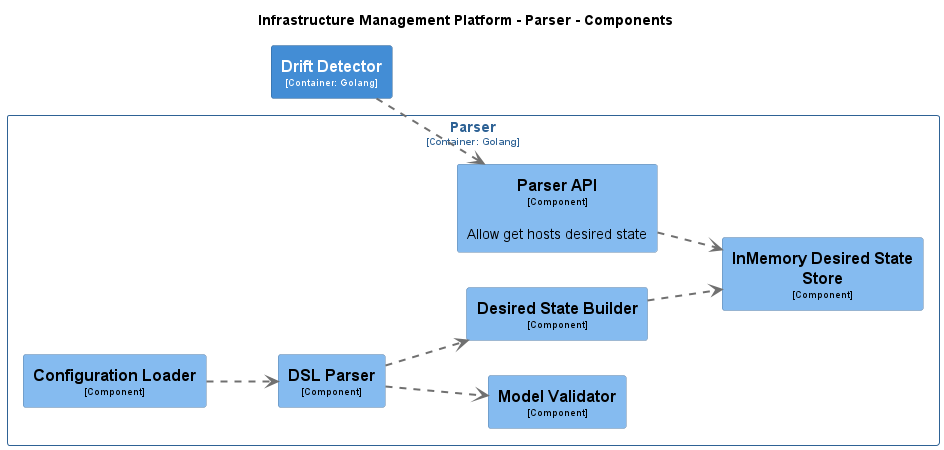
\includegraphics[width=0.95\linewidth]{../platform-arch-images/parser-components.png}
  \caption{Компонентная структура ParserSvc}
  \label{fig:ch3-parser-components}
\end{figure}

На уровне запуска сервис выполняет последовательность действий: загружает конфигурацию, определяет путь к манифестам, находит доступные JSON-файлы, разбирает каждый валидный файл, строит desired state и сохраняет его во внутреннем in-memory store. После этого поднимается HTTP API, через которое остальные компоненты платформы получают целевое состояние.

Конфигурация сервиса содержит параметры HTTP-сервера, уровень логирования и блок \texttt{manifests}. Для манифестов поддерживаются два режима: \texttt{file} и \texttt{directory}. В режиме \texttt{file} сервис обрабатывает один указанный файл. В режиме \texttt{directory} он просматривает верхний уровень директории и выбирает только файлы с расширением \texttt{.json}. Файлы с другими расширениями, включая \texttt{.dsl}, игнорируются. Такое решение связано с тем, что ParserSvc не является интерпретатором Structurizr DSL; он работает со структурированным JSON-представлением.

Разбор входного файла выполняется в два этапа. Сначала JSON десериализуется во внутреннюю структуру Structurizr-манифеста. Сервис проверяет наличие \texttt{model.deploymentNodes}, поскольку без deployment-узлов невозможно построить host-centric desired state. Затем mapper-слой преобразует элементы Structurizr-модели в доменную модель платформы.

Для сопоставления container instance с именем workload mapper строит карту контейнеров по \texttt{containerId}. Источником этой карты служит раздел \texttt{model.softwareSystems[].containers}. Далее сервис рекурсивно обходит deployment-узлы. Это важно, потому что Structurizr-модель может содержать вложенные deployment node, а инфраструктурно значимые хосты не всегда находятся только на верхнем уровне.

Для каждого deployment node извлекаются обязательные свойства: \texttt{host\_id}, \texttt{fqdn}, \texttt{env}, \texttt{managed\_by}, \texttt{purpose}. Поле \texttt{ip} является необязательным. Остальные свойства, не относящиеся к служебным полям Structurizr, преобразуются в labels. Таким образом, desired state сохраняет как минимально обязательные атрибуты, так и дополнительные признаки хоста: регион, владельца, роль или иные эксплуатационные метки.

Workload строится на основе container instance. Обязательными полями являются имя контейнера, \texttt{enabled} и \texttt{deployment\_mode}. Если режим развертывания равен \texttt{container}, обязательным становится поле \texttt{image}. Дополнительно поддерживаются \texttt{version} и \texttt{port}.

Итоговое состояние сохраняется в in-memory store как snapshot. Store возвращает копии данных, что защищает внутреннее состояние от случайного изменения вызывающим кодом. В metadata snapshot фиксируются время загрузки, режим и путь манифестов, количество найденных, загруженных, поврежденных и проигнорированных файлов, общее число хостов и workload, а также readiness-статус.

HTTP API ParserSvc включает:
\begin{enumerate}
    \item \texttt{GET /healthz} --- проверка liveness;
    \item \texttt{GET /readyz} --- проверка готовности desired state;
    \item \texttt{GET /api/v1/desired-state} --- получение полного desired state;
    \item \texttt{GET /api/v1/desired-state/hosts} --- получение списка хостов с фильтрами;
    \item \texttt{GET /api/v1/desired-state/hosts/:hostId} --- получение одного хоста по идентификатору.
\end{enumerate}

Список хостов поддерживает фильтрацию по \texttt{fqdn} и labels. Несколько фильтров применяются с AND-семантикой. Это полезно для последующего расширения платформы, поскольку позволяет выбирать хосты по окружению, команде, назначению или другим признакам без изменения внутренней модели desired state.

\subsection{Реализация InventorySvc: selfProvisioning, cAdvisor, snapshot, partial result}

\texttt{InventorySvc} реализован на Go и отвечает за формирование actual state управляемых хостов. Компонентная структура сервиса представлена на рисунке~\ref{fig:ch3-inventory-components}.

\begin{figure}
  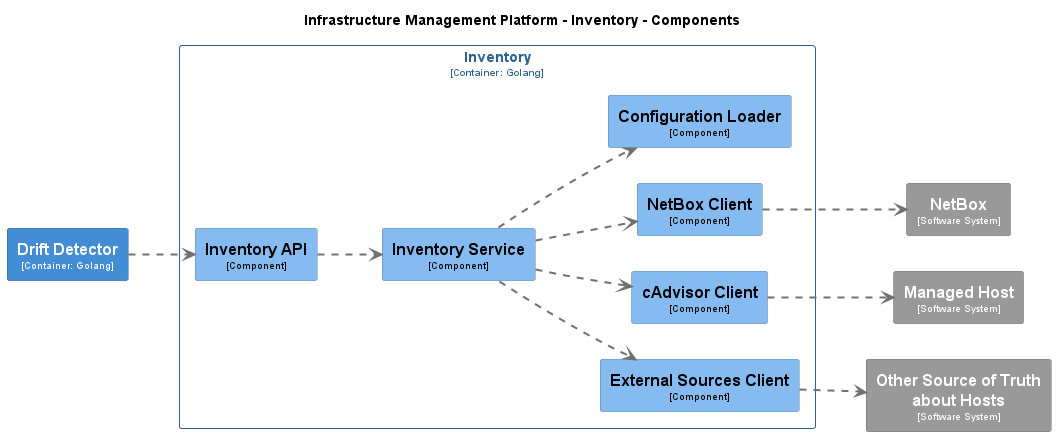
\includegraphics[width=0.95\linewidth]{../platform-arch-images/inventory-components.png}
  \caption{Компонентная структура InventorySvc}
  \label{fig:ch3-inventory-components}
\end{figure}

Сервис построен как canonical read-model фактического состояния. Он не обращается к cAdvisor при каждом HTTP-запросе. Вместо этого InventorySvc периодически выполняет синхронизацию, формирует snapshot и отдаёт через API уже подготовленные данные. Такой подход уменьшает зависимость потребителей API от мгновенной доступности внешних источников и делает ответы согласованными в пределах завершенного цикла синхронизации.

Начальная область наблюдения задается файлом \texttt{selfProvisioning}. Он содержит список хостов с полями \texttt{id}, \texttt{fqdn} и \texttt{labels}. Валидация требует уникальности \texttt{id} и \texttt{fqdn}, а также наличия обязательных labels: \texttt{managed\_by}, \texttt{purpose}, \texttt{env}. Таким образом, bootstrap-описание задает минимальную инвентарную основу, от которой сервис отталкивается при сборе actual state.

Фактические сведения о workload собираются через source-слой. Для каждого bootstrap-хоста сервис строит URL по шаблону из конфигурации и обращается к endpoint \texttt{/api/v1.3/subcontainers/}. Ответ cAdvisor нормализуется в доменную модель \texttt{Workload}. При этом из данных контейнера выделяются идентификатор, имя, image, runtime, источник и время последнего наблюдения.

Синхронизация InventorySvc выполняется как initial sync и periodic sync. Initial sync происходит до перехода сервиса в состояние ready. Periodic sync запускается по интервалу из конфигурации и обновляет snapshot. Внутреннее хранилище использует потокобезопасный доступ, поэтому API может читать предыдущее согласованное состояние, пока очередной цикл синхронизации готовит новое.

Особое внимание в реализации уделено partial result. Если источник данных недоступен для части хостов, InventorySvc не завершает работу ошибкой и не отбрасывает полностью результат синхронизации. Вместо этого он возвращает данные по доступным хостам, а для проблемных хостов фиксирует ошибки и статусы источников. На уровне metadata выставляются признаки \texttt{isPartial}, \texttt{failedHosts}, \texttt{lastSyncAt}, \texttt{lastFullSyncAt} и \texttt{lastPartialSyncAt}.

Статус хоста может принимать значения \texttt{ok}, \texttt{partial}, \texttt{error}, \texttt{bootstrap\_only}. Дополнительно для каждого источника хранится \texttt{sourceStatus}: включен ли источник, успешно ли он отработал, когда были получены данные и какая ошибка возникла при неуспехе. Именно эта информация затем используется DriftDetectorSvc для безопасного решения: можно ли считать actual state достаточно полным для обнаружения drift.

HTTP API InventorySvc включает:
\begin{enumerate}
    \item \texttt{GET /healthz} --- проверка liveness;
    \item \texttt{GET /readyz} --- проверка готовности после initial sync;
    \item \texttt{GET /api/v1/hosts} --- список хостов с metadata;
    \item \texttt{GET /api/v1/hosts/:id} --- карточка одного хоста.
\end{enumerate}

Список хостов поддерживает фильтрацию по labels с AND-семантикой. API возвращает не только workload, но и metadata snapshot, что позволяет потребителю учитывать полноту actual state. Для платформы это принципиально: качество решения о drift зависит не только от списка workload, но и от того, насколько достоверны данные источника.

\subsection{Реализация DriftDetectorSvc: клиенты, detector registry, cooldown, статистика цикла}

\texttt{DriftDetectorSvc} реализован на Go и является компонентом, который связывает desired state, actual state и reconcile. Его компонентная структура представлена на рисунке~\ref{fig:ch3-drift-detector-components}.

\begin{figure}
  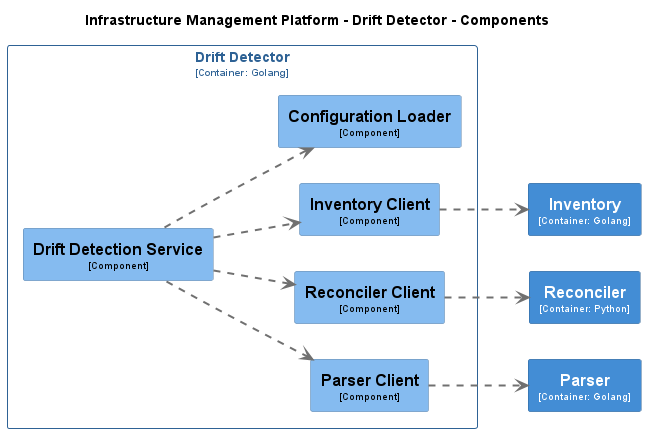
\includegraphics[width=0.95\linewidth]{../platform-arch-images/drift-detector-components.png}
  \caption{Компонентная структура DriftDetectorSvc}
  \label{fig:ch3-drift-detector-components}
\end{figure}

При запуске сервис загружает конфигурацию, инициализирует HTTP-клиенты для ParserSvc, InventorySvc и ReconcilerSvc, создает registry detector-ов и запускает первый detection cycle. После успешного цикла сервис считается ready. Дополнительно поддерживается периодический запуск по scheduler и ручной запуск одного цикла через API.

Detection cycle выполняется последовательно. Сначала сервис получает actual state, затем desired state. После этого он индексирует actual-хосты по \texttt{host\_id} и \texttt{fqdn}. Для каждого desired-хоста выполняется поиск соответствующего actual-хоста. Приоритет отдается \texttt{host\_id}; если он не найден, используется \texttt{fqdn}. Если хост не найден, цикл помечается как partial, а данный хост пропускается.

Далее для каждого включенного компонента вызывается соответствующий detector. Каждый detector реализует общий интерфейс и возвращает структурированный результат: применима ли проверка, отсутствуют ли actual-данные, найден ли drift, какое предупреждение сформировано и какую reconcile-команду следует отправить.

Detector \texttt{cadvisor} имеет особую bootstrap-семантику. Если desired state требует \texttt{cadvisor}, но источник cAdvisor для хоста недоступен, detector может сформировать reconcile-команду на установку cAdvisor. Такое поведение оправдано тем, что cAdvisor является не только управляемым workload, но и источником actual state для последующих проверок.

После обнаружения drift DriftDetectorSvc формирует reconcile-команду. В команду входят \texttt{host\_id}, \texttt{fqdn}, \texttt{component}, \texttt{correlation\_id} и параметры компонента. Для \texttt{node\_exporter} это могут быть \texttt{node\_exporter\_image} и \texttt{node\_exporter\_port}; для \texttt{cadvisor} --- \texttt{cadvisor\_image} и \texttt{cadvisor\_port}. \texttt{correlation\_id} строится из идентификатора detection cycle, компонента и FQDN, что упрощает трассировку действий в логах.

Перед отправкой команды применяется cooldown-хранилище. Оно реализовано как in-memory map вида \texttt{component|fqdn -> lastSentAt}. Если с момента последней отправки прошло меньше заданного интервала, команда подавляется. В статистике цикла увеличивается счетчик \texttt{reconcileSuppressed}. Если отправка разрешена и ReconcilerSvc вернул \texttt{202 Accepted}, команда считается принятой, а ключ cooldown обновляется.

Результат каждого цикла сохраняется как \texttt{DetectionCycleResult}. В нем фиксируются идентификатор цикла, trigger, время начала и завершения, длительность, stage timings, признаки partial, готовность ParserSvc, статистика и списки предупреждений/ошибок. Stage timings включают время получения inventory, время получения desired state, время сравнения drift и время отправки reconcile-команд.

HTTP API DriftDetectorSvc включает:
\begin{enumerate}
    \item \texttt{GET /healthz} --- liveness;
    \item \texttt{GET /readyz} --- readiness на основе успешного detection cycle;
    \item \texttt{POST /api/v1/detection/run} --- запуск одного detection cycle.
\end{enumerate}

Для ручного запуска реализована защита от параллельного выполнения. Если detection cycle уже идет, сервис возвращает \texttt{409 Conflict}. Это важно для согласованности статистики и для предотвращения одновременной отправки одинаковых reconcile-команд.

\subsection{Реализация ReconcilerSvc: FastAPI, очередь, operators, Ansible Runner}

\texttt{ReconcilerSvc} реализован на Python с использованием FastAPI. Сервис принимает reconcile-команды, валидирует их, выбирает operator, строит execution plan и ставит задачу во внутреннюю очередь. Компонентная структура сервиса представлена на рисунке~\ref{fig:ch3-reconciler-components}.

\begin{figure}
  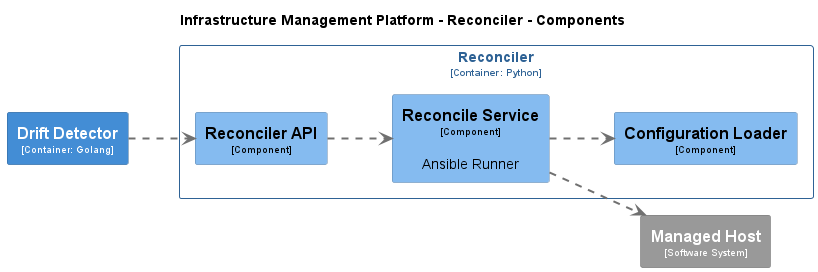
\includegraphics[width=0.95\linewidth]{../platform-arch-images/reconciler-components.png}
  \caption{Компонентная структура ReconcilerSvc}
  \label{fig:ch3-reconciler-components}
\end{figure}

HTTP API сервиса содержит \texttt{GET /healthz}, \texttt{GET /readyz} и \texttt{POST /api/v1/reconcile}. Основной запрос описан моделью \texttt{ReconcileRequest}. Обязательными полями являются \texttt{fqdn} и \texttt{component}. Дополнительно могут передаваться \texttt{host\_id}, \texttt{correlation\_id} и словарь \texttt{parameters}. Для FQDN выполняется валидация допустимых символов.

При успешном принятии запроса сервис возвращает \texttt{ReconcileAcceptedResponse} со статусом \texttt{accepted}, \texttt{request\_id}, компонентом, FQDN, \texttt{correlation\_id} и временем принятия. Важно, что ответ \texttt{202 Accepted} означает только постановку задачи в очередь. Он не означает, что workload уже установлен или что Ansible playbook завершился успешно.

Основная бизнес-логика сосредоточена в \texttt{ReconcileService}. Сервис генерирует \texttt{request\_id}, логирует входящий запрос, выбирает operator через \texttt{OperatorRegistry}, строит execution plan и передает задачу в очередь. Если очередь переполнена или не готова принимать задачи, API возвращает \texttt{503}. Если operator не найден, возвращается ошибка клиентского запроса. Если execution plan не может быть построен, возвращается серверная ошибка.

Operator-слой состоит из базового интерфейса \texttt{ReconcileOperator}, registry и конкретных operator-ов. Каждый operator знает, какой playbook использовать и какие default parameters применить. При построении execution plan default-параметры объединяются с параметрами, полученными от DriftDetectorSvc. Это позволяет detector-у передать image или port из desired state, не меняя общий контракт ReconcilerSvc.

Выполнение playbook изолировано в \texttt{AnsibleRunnerAdapter}. Adapter читает SSH-параметры из переменных окружения, строит in-memory inventory для целевого FQDN, добавляет служебные extra vars и запускает Ansible Runner \cite{ansible_docs}. Результат выполнения нормализуется до статуса, кода возврата, признака успешности и длительности. Потоковые события Ansible логируются со служебными полями \texttt{request\_id}, \texttt{component}, \texttt{fqdn} и \texttt{correlation\_id}.

Таким образом, ReconcilerSvc реализует управляемую асинхронную модель восстановления. Он отделяет прием команды от выполнения, ограничивает параллелизм, скрывает детали Ansible за adapter-слоем и предоставляет точку расширения через operator registry.

\subsection{Контракты API и взаимодействие сервисов}

Взаимодействие сервисов построено на явных HTTP-контрактах. Такой подход делает границы компонентов прозрачными и позволяет развивать внутреннюю реализацию сервисов без изменения их внешнего поведения.

Общий поток взаимодействия можно описать следующим образом. ParserSvc заранее формирует desired state из Structurizr JSON. InventorySvc формирует actual state на основе bootstrap-описания и данных источников наблюдения. DriftDetectorSvc обращается к обоим сервисам, нормализует полученные ответы в собственные доменные модели и применяет detector-ы. При подтвержденном drift DriftDetectorSvc отправляет reconcile-команду в ReconcilerSvc. ReconcilerSvc принимает команду, строит execution plan и асинхронно выполняет восстановление через Ansible Runner.

Проектная особенность состоит в том, что ни один сервис не обращается напрямую к внутреннему состоянию другого сервиса. ParserSvc и InventorySvc скрывают свои in-memory snapshot за API. DriftDetectorSvc не знает, как именно ParserSvc разбирает Structurizr JSON и как InventorySvc получает данные от cAdvisor. ReconcilerSvc не знает, по каким правилам был обнаружен drift; он работает с уже сформированной reconcile-командой.

Такая организация дает несколько инженерных преимуществ. Во-первых, упрощается тестирование: каждый сервис можно проверять через его публичные функции и HTTP-слой. Во-вторых, появляется возможность независимого расширения. Например, InventorySvc может получить новый источник данных, не меняя DriftDetectorSvc, если внешний контракт actual state сохранится. В-третьих, повышается надежность границ: ошибки получения actual state, ошибки разбора desired state и ошибки выполнения reconcile фиксируются в разных местах и не смешиваются в один монолитный процесс.

Итогом реализации стала связанная платформа, в которой каждый компонент выполняет собственную роль в общем цикле управления инфраструктурой. ParserSvc предоставляет целевое состояние из архитектурного описания, InventorySvc предоставляет наблюдаемое состояние, DriftDetectorSvc принимает решение о расхождении, а ReconcilerSvc выполняет восстановление поддержанных workload. В следующей главе рассматривается проверка качества разработанного решения и экспериментальная оценка ключевых характеристик платформы.

    \section{ИССЛЕДОВАНИЕ И ОЦЕНКА КАЧЕСТВА РАЗРАБОТАННОГО РЕШЕНИЯ}

После реализации компонентов платформы необходимо проверить, что полученное решение соответствует поставленной задаче и корректно выполняет ключевой цикл управления: построение desired state, получение actual state, обнаружение drift и запуск reconcile. Оценка качества в данной работе выполняется по двум направлениям. Первое направление связано с тестированием отдельных сервисов и их доменной логики. Второе направление связано с экспериментальной оценкой поведения платформы на сценариях, отражающих основные эксплуатационные свойства: масштабируемость detection cycle, время сходимости после drift, пропускную способность reconcile, устойчивость к partial data и эффективность cooldown.

\subsection{Цели, критерии и ограничения испытаний}

Главная цель испытаний --- подтвердить, что разработанная платформа реализует заявленную архитектурную модель. Для этого необходимо проверить, что каждый сервис корректно выполняет собственную функцию, а цепочка сервисов в совокупности обеспечивает обнаружение и устранение поддержанного drift.

Критерии оценки сформулированы следующим образом:
\begin{enumerate}
    \item ParserSvc должен корректно загружать Structurizr JSON, валидировать данные и строить desired state;
    \item InventorySvc должен корректно формировать actual state, поддерживать snapshot и явно отражать partial result;
    \item DriftDetectorSvc должен корректно сопоставлять desired state и actual state, обнаруживать drift только при достаточных данных и подавлять повторные reconcile-команды в пределах cooldown;
    \item ReconcilerSvc должен принимать reconcile-команды, валидировать payload, выбирать operator, строить execution plan и ставить задачу в очередь;
    \item API-контракты сервисов должны быть согласованы с фактическими структурами данных;
    \item экспериментальные сценарии должны демонстрировать работоспособность control loop и позволять оценить узкие места MVP.
\end{enumerate}

Испытания имеют несколько ограничений. Во-первых, текущая версия платформы поддерживает только два компонента: \texttt{node\_exporter} и \texttt{cadvisor}. Следовательно, результаты нельзя напрямую переносить на произвольные workload без реализации дополнительных detector-ов и operator-ов. Во-вторых, состояние cooldown, desired state и actual state хранится в памяти, поэтому верификация не охватывает сценарии восстановления после перезапуска с сохранением истории. В-третьих, измерения производительности не являются SLA: они отражают поведение MVP в выбранных условиях и служат инженерной точкой отсчета для последующих оптимизаций.

Отдельно важно зафиксировать ограничение partial data. В платформе отсутствие фактических данных не должно автоматически считаться drift. Поэтому в испытаниях проверяется не только способность обнаруживать расхождения, но и способность не выполнять лишние reconcile-действия при неполной информации.

\subsection{Модульные и компонентные тесты}

Тестовый контур охватывает все основные сервисы платформы. Для Go-сервисов используются unit-тесты, расположенные рядом с соответствующими пакетами. Для ReconcilerSvc используются Python-тесты на базе pytest. Такой подход соответствует структуре проекта: каждый сервис проверяется в собственной технологической среде и на уровне собственных доменных компонентов.

В ParserSvc тестируются загрузка конфигурации, обнаружение manifest-файлов, разбор Structurizr JSON, mapping deployment-модели в desired state, валидация workload и host-полей, in-memory store и HTTP handlers. Эти тесты подтверждают, что сервис корректно обрабатывает валидные манифесты, пропускает некорректные элементы и поддерживает фильтрацию desired-хостов.

В InventorySvc проверяются загрузка конфигурации, валидация selfProvisioning, mapping ответа cAdvisor, фильтрация системных workload, потокобезопасное поведение in-memory store, фильтрация хостов по labels и HTTP handlers. Особое значение имеют тесты cAdvisor mapper: они подтверждают, что сервис выделяет из внешнего ответа именно workload, которые затем могут использоваться DriftDetectorSvc для сравнения с desired state.

В DriftDetectorSvc тестируются конфигурация, HTTP-клиенты ParserSvc, InventorySvc и ReconcilerSvc, detector registry, detector-ы для \texttt{node\_exporter} и \texttt{cadvisor}, cooldown store, scheduler, HTTP handlers и основной detection service. Набор тестов включает проверку обнаружения отсутствующего компонента, отсутствие drift при наличии workload, bootstrap-поведение для \texttt{cadvisor}, подавление повторных reconcile-команд, partial-обработку при отсутствующем actual host и запрет параллельного запуска detection cycle.

В ReconcilerSvc тестируются схемы Pydantic, API endpoints, operator registry, построение execution plan, очередь задач, reconcile service и Ansible adapter с подменой runner-а. Эти тесты подтверждают, что сервис корректно валидирует входные данные, возвращает \texttt{202 Accepted} при успешной постановке в очередь, возвращает \texttt{503} при насыщении очереди и строит корректный in-memory inventory для Ansible Runner.

\begin{table}
    \centering
    \caption{Основные группы тестов компонентов платформы}
    \label{tab:ch4-test-groups}
    \footnotesize
    \begin{tabularx}{\textwidth}{|p{0.22\textwidth}|X|}\hline
    Сервис & Проверяемые аспекты \\ \hline
    ParserSvc & Конфигурация, поиск JSON-манифестов, разбор Structurizr JSON, mapping desired state, валидация, store, API handlers \\ \hline
    InventorySvc & Конфигурация, selfProvisioning, cAdvisor client/mapper, фильтрация workload, in-memory snapshot, labels filtering, API handlers \\ \hline
    DriftDetectorSvc & HTTP-клиенты, detector registry, detector-ы, cooldown, detection cycle, scheduler, partial-обработка, API handlers \\ \hline
    ReconcilerSvc & Pydantic-схемы, API, operator registry, execution plan, очередь, reconcile service, Ansible adapter \\ \hline
    \end{tabularx}
    \normalsize
\end{table}

Таким образом, модульные и компонентные тесты покрывают наиболее рискованные участки реализации: преобразование данных между форматами, принятие решения о drift, подавление повторных действий и асинхронную постановку reconcile-задач. Это создает основу для дальнейшей экспериментальной оценки поведения платформы как единой системы.

\subsection{Методика экспериментальной оценки}

Экспериментальная оценка выполнялась набором сценариев, которые проверяют не отдельные функции сервисов, а поведение платформы как связанного control loop. Для этого использовались HTTP API сервисов, структурированные логи и сохраненные артефакты выполнения.

Методика включает пять сценариев:
\begin{enumerate}
    \item оценка масштабируемости detection cycle при различном числе управляемых хостов;
    \item оценка времени сходимости после внесения drift;
    \item оценка пропускной способности ReconcilerSvc и поведения при насыщении очереди;
    \item проверка устойчивости при partial data;
    \item оценка эффективности cooldown для подавления повторных reconcile-команд.
\end{enumerate}

Для каждого сценария собирались сырые результаты в JSON и сводный отчет. В качестве метрик использовались длительность detection cycle, длительности отдельных стадий цикла, количество найденных drift, количество отправленных и подавленных reconcile-команд, число принятых и отклоненных reconcile-запросов, throughput завершения reconcile-задач и признаки partial-обработки.

Важная особенность методики состоит в разделении стадий detection cycle. Для анализа недостаточно знать только полную длительность цикла. Необходимо понимать, какая часть времени приходится на получение inventory, какая --- на получение desired state, какая --- на сравнение, а какая --- на dispatch reconcile-команд. Поэтому DriftDetectorSvc сохраняет stage timings: \texttt{InventoryFetchMs}, \texttt{ParserFetchMs}, \texttt{DriftComparisonMs}, \texttt{ReconcileDispatchMs}.

\subsection{Масштабируемость detection cycle}

Первый сценарий направлен на оценку того, как длительность detection cycle изменяется при росте числа управляемых хостов. В сценарии рассматривались случаи с 1, 10, 100 и 500 хостами. Для каждого случая выполнялось несколько циклов в устойчивом состоянии, когда reconcile dispatch отсутствовал. Это позволяет оценивать именно стоимость получения и сравнения состояний, а не стоимость восстановления workload.

\begin{table}
    \centering
    \caption{Результаты оценки масштабируемости detection cycle}
    \label{tab:ch4-detection-scalability}
    \footnotesize
    \begin{tabular}{|r|r|r|r|r|r|r|}\hline
    Хосты & Cycle p50, мс & Inventory p50, мс & Parser p50, мс & Compare p50, мс & Dispatch p50, мс \\ \hline
    1   & 0.0  & 0.0  & 0.0 & 0.0 & 0.0 \\ \hline
    10  & 1.0  & 0.0  & 0.0 & 0.0 & 0.0 \\ \hline
    100 & 6.0  & 3.0  & 2.0 & 0.0 & 0.0 \\ \hline
    500 & 20.0 & 12.0 & 6.0 & 0.0 & 0.0 \\ \hline
    \end{tabular}
    \normalsize
\end{table}

Данные таблицы~\ref{tab:ch4-detection-scalability} показывают, что рост длительности цикла в основном связан с увеличением времени получения actual state и desired state. Для 100 хостов медианная длительность цикла составила 6 мс, для 500 хостов --- 20 мс. При этом медианное время стадии сравнения округлялось к 0 мс, что показывает низкую стоимость самой логики сопоставления в сравнении с fetch-стадиями.

Отсутствие dispatch-времени объясняется тем, что измеренные циклы выполнялись в состоянии без новых reconcile-команд. Это важно для корректной интерпретации: сценарий оценивает масштабирование detection logic, а не производительность ReconcilerSvc.

Полученный результат подтверждает, что в текущей реализации основная стоимость detection cycle при росте числа хостов связана с получением данных от сервисов-источников. Следовательно, дальнейшие оптимизации масштабируемости должны быть направлены прежде всего на ускорение InventorySvc/ParserSvc API, кэширование, уменьшение объема передаваемых данных или введение более точных инкрементальных механизмов.

\subsection{Время сходимости после drift}

Второй сценарий оценивает время сходимости после искусственного появления drift. Под сходимостью понимается интервал от момента внесения расхождения до момента восстановления требуемого workload и последующего исчезновения drift в наблюдаемом состоянии.

В измеренном сценарии удалялся workload \texttt{node\_exporter}. Далее фиксировались ключевые интервалы: время до первого detection cycle, время от обнаружения до отправки reconcile-команды, время выполнения восстановления и полное время сходимости.

\begin{table}
    \centering
    \caption{Время сходимости после drift}
    \label{tab:ch4-convergence-time}
    \footnotesize
    \begin{tabularx}{0.8\textwidth}{|X|r|}\hline
    Метрика & Значение, мс \\ \hline
    Inject -> first detection & 4075 \\ \hline
    Detection -> reconcile send & 4 \\ \hline
    Reconcile send -> workload restored & 10219 \\ \hline
    Total convergence & 14300 \\ \hline
    \end{tabularx}
    \normalsize
\end{table}

Как видно из таблицы~\ref{tab:ch4-convergence-time}, полное время сходимости составило 14300 мс. При этом собственно отправка reconcile-команды после обнаружения drift заняла 4 мс. Основная часть времени пришлась на выполнение восстановления и ожидание обновления actual state.

Такой результат согласуется с архитектурой платформы. DriftDetectorSvc быстро принимает решение и передает команду ReconcilerSvc, но фактическое восстановление зависит от выполнения Ansible playbook и последующего появления обновленных данных в inventory snapshot. Следовательно, время сходимости определяется не только скоростью detection cycle, но и длительностью reconcile execution, частотой обновления inventory и задержками источников actual state.

Практический вывод состоит в том, что для сокращения convergence latency необходимо оптимизировать несколько участков одновременно. Уменьшение интервала detection само по себе не даст полного эффекта, если reconcile playbook выполняется долго или actual state обновляется редко. В дальнейшем полезно добавить явные события о завершении reconcile и более точное отслеживание момента восстановления workload.

\subsection{Throughput reconcile и насыщение очереди}

Третий сценарий направлен на проверку ReconcilerSvc. В нем оценивалось, как меняется throughput завершения reconcile-задач при разных значениях параллелизма, а также как сервис ведет себя при burst-нагрузке.

\begin{table}
    \centering
    \caption{Результаты оценки reconcile throughput}
    \label{tab:ch4-reconcile-throughput}
    \footnotesize
    \begin{tabular}{|p{0.28\textwidth}|r|r|r|r|r|r|}\hline
    Сценарий & Parallelism & Requests & Accepted & Rejected & Success & Ops/s \\ \hline
    steady\_parallel\_1 & 1 & 90  & 90  & 0  & 90 & 0.2392 \\ \hline
    steady\_parallel\_2 & 2 & 90  & 90  & 0  & 81 & 0.4636 \\ \hline
    steady\_parallel\_4 & 4 & 90  & 90  & 0  & 83 & 0.7822 \\ \hline
    saturation\_probe\_parallel\_2 & 2 & 180 & 102 & 78 & 99 & 0.4579 \\ \hline
    \end{tabular}
    \normalsize
\end{table}

Результаты таблицы~\ref{tab:ch4-reconcile-throughput} показывают ожидаемую зависимость: при увеличении \texttt{max\_parallel\_reconciliations} throughput завершения возрастает.

Отдельный интерес представляет сценарий saturation. При 180 запросах и параллелизме 2 сервис принял 102 запроса и отклонил 78. Это подтверждает, что ограничение очереди работает: ReconcilerSvc не принимает неограниченное число задач, а возвращает \texttt{503}, когда очередь не может принять новую задачу в заданный timeout. С точки зрения надежности это предпочтительнее бесконтрольного накопления задач и роста задержек.

Следует учитывать, что число successful completions в некоторых сценариях меньше числа accepted. Это отражает асинхронную природу выполнения и ограниченное окно наблюдения за завершением задач. Для более точной production-оценки в дальнейшем требуется persisted job state и отдельный API статуса очереди, чтобы различать принятые, выполняемые, завершенные и ошибочные задачи.

Таким образом, текущая реализация ReconcilerSvc демонстрирует управляемое поведение под нагрузкой. Worker pool позволяет масштабировать параллелизм, а queue capacity задает верхнюю границу накопления задач. Главным узким местом остается выполнение Ansible playbook, что ожидаемо для agentless-модели восстановления через SSH.

\subsection{Устойчивость к partial data и эффективность cooldown}

Четвертый и пятый сценарии проверяют безопасность автоматических действий. Для инфраструктурной платформы важно не только уметь устранять drift, но и не выполнять лишние действия при неполных данных или повторяющихся сигналах.

В сценарии partial data рассматривалась ситуация, когда часть хостов недоступна для получения actual state. В измерении использовалось 20 хостов, из которых 6 имели недоступные FQDN для InventorySvc. Результаты приведены в таблице~\ref{tab:ch4-partial-data}.

\begin{table}
    \centering
    \caption{Результаты проверки устойчивости к partial data}
    \label{tab:ch4-partial-data}
    \footnotesize
    \begin{tabularx}{0.85\textwidth}{|X|r|}\hline
    Метрика & Значение \\ \hline
    Cycle partial flag & true \\ \hline
    Inventory \texttt{metadata.isPartial} & true \\ \hline
    Inventory \texttt{failedHosts} & 6 \\ \hline
    Warnings: missing actual data & 6 \\ \hline
    Node exporter reconciles for missing hosts & 0 \\ \hline
    Cadvisor reconciles for missing hosts & 0 \\ \hline
    \end{tabularx}
    \normalsize
\end{table}

Полученные значения подтверждают корректную partial-семантику. DriftDetectorSvc продолжил обработку доступных данных, но не стал автоматически отправлять reconcile-команды для хостов с недостоверным actual state. Для отсутствующих данных были зафиксированы предупреждения, а цикл был помечен как partial. Это соответствует требованию безопасности: неполнота данных не должна превращаться в основание для произвольного восстановления.

Сценарий cooldown проверял подавление повторных reconcile-команд. Он моделировал повторяющийся drift в нескольких циклах. Результаты приведены в таблице~\ref{tab:ch4-cooldown}.

\begin{table}
    \centering
    \caption{Результаты проверки эффективности cooldown}
    \label{tab:ch4-cooldown}
    \footnotesize
    \begin{tabularx}{0.85\textwidth}{|X|r|}\hline
    Метрика & Значение \\ \hline
    Reconcile sent without cooldown & 20 \\ \hline
    Reconcile sent with cooldown & 0 \\ \hline
    Prevented reconcile commands & 20 \\ \hline
    Suppression ratio & 1.0 \\ \hline
    \end{tabularx}
    \normalsize
\end{table}

Результаты показывают, что cooldown полностью подавил повторные отправки в рамках окна эксперимента. Это важно для устойчивости платформы. Если drift не может быть устранен сразу, повторная отправка одинаковых команд в каждом цикле привела бы к перегрузке ReconcilerSvc и управляемых хостов. Cooldown снижает этот риск и делает поведение системы более предсказуемым.

Вместе с тем текущая реализация cooldown хранит состояние в памяти DriftDetectorSvc. Следовательно, при перезапуске сервиса история подавления теряется. Для более зрелой эксплуатации необходимо вынести cooldown/history в персистентное хранилище или отдельный механизм deduplication.

\subsection{Интерпретация результатов и ограничения измерений}

Проведенные испытания показывают, что разработанная платформа выполняет ключевые функции MVP. ParserSvc корректно строит desired state из архитектурного JSON-представления, InventorySvc формирует actual state и явно отражает partial result, DriftDetectorSvc обнаруживает поддержанные виды drift и подавляет повторные reconcile-команды, а ReconcilerSvc принимает команды и выполняет их через асинхронную очередь и operator-слой.

Экспериментальная оценка подтверждает несколько важных свойств. Во-первых, detection cycle масштабируется предсказуемо для проверенного диапазона хостов, а основная стоимость роста связана с получением данных от сервисов-источников. Во-вторых, время сходимости после drift определяется не только скоростью обнаружения, но и длительностью reconcile и обновления actual state. В-третьих, ReconcilerSvc демонстрирует управляемое поведение под нагрузкой: рост параллелизма повышает throughput, а насыщение очереди приводит к отказу в приеме новых задач вместо неконтролируемого накопления. В-четвертых, partial data и cooldown работают как защитные механизмы от ошибочных или избыточных действий.

Ограничения измерений также существенны. Сценарии с 100 и 500 хостами отражают масштабирование control-plane-логики, а не полноценную эксплуатацию сотен независимых физических узлов. Абсолютные значения задержек зависят от вычислительных ресурсов, конфигурации сервисов, особенностей Ansible-выполнения и способа моделирования данных. Кроме того, stage timing для очень быстрых стадий может округляться до 0 мс, поэтому такие значения следует интерпретировать как признак малой длительности, а не как буквальное отсутствие затрат.

На основе результатов можно выделить направления улучшения качества. Для detection cycle полезно добавить более подробные метрики по стадиям и объемам данных. Для ReconcilerSvc необходим API статуса очереди и persisted job history. Для cooldown и истории drift требуется персистентное состояние. Для convergence-оценки полезен явный event о восстановлении workload, чтобы уменьшить зависимость измерений от периодического получения actual state.

Таким образом, глава подтверждает, что разработанное решение является работоспособным MVP автоматизированной платформы управления инфраструктурой с поддержкой Architecture-as-Code. Оно реализует основной control loop и демонстрирует ожидаемое поведение в ключевых сценариях, при этом имеет понятные ограничения и направления дальнейшего развития.

    \section{ПРАКТИЧЕСКАЯ АПРОБАЦИЯ, ОГРАНИЧЕНИЯ И НАПРАВЛЕНИЯ РАЗВИТИЯ}

После проектирования, реализации и экспериментальной оценки необходимо определить, какую практическую задачу решает разработанная платформа, где проходят границы текущего MVP и какие направления развития являются наиболее важными. Данная глава связывает технические результаты предыдущих разделов с эксплуатационным смыслом работы: снижением ручной нагрузки на инженеров и повышением наблюдаемости состояния инфраструктуры.

\subsection{Практическая апробация разработанной платформы}

Практическая апробация выполнялась на сценарии управления контейнерными workload, который отражает основную идею работы. В архитектурном описании задается управляемый хост и два требуемых компонента: \texttt{node\_exporter} и \texttt{cadvisor}. ParserSvc преобразует это описание в desired state, где для каждого workload указаны имя, признак включения, режим развертывания, image и port. InventorySvc формирует actual state, получая сведения о фактически наблюдаемых контейнерных workload. DriftDetectorSvc сравнивает состояния и при подтвержденном расхождении отправляет reconcile-команду в ReconcilerSvc.

Сценарий выбран не случайно. \texttt{node\_exporter} и \texttt{cadvisor} относятся к инфраструктурным компонентам наблюдаемости. Такие workload часто должны присутствовать на управляемых хостах, но их отсутствие не всегда сразу заметно прикладным командам. Если агент или контейнер наблюдаемости пропал, эксплуатационная команда может потерять часть метрик и обнаружить проблему уже после того, как понадобится диагностика инцидента. Поэтому автоматическое обнаружение отсутствующего компонента и запуск восстановления имеют понятную практическую ценность.

В ходе апробации подтверждено, что платформа реализует полный путь данных. Desired state формируется из Structurizr JSON, а не задается вручную внутри DriftDetectorSvc. Actual state поступает через InventorySvc и содержит не только список workload, но и metadata о полноте данных. DriftDetectorSvc учитывает эту полноту и не отправляет reconcile-команды при недостоверном actual state, кроме специально предусмотренного bootstrap-сценария для \texttt{cadvisor}. ReconcilerSvc принимает команду асинхронно и передает выполнение operator-слою.

Отдельный результат апробации связан с partial-семантикой. В инфраструктурной автоматизации ошибочное действие может быть опаснее бездействия. Поэтому платформа должна уметь признавать неполноту данных и не превращать сетевую ошибку или недоступность источника в автоматический reconcile. Проверенный сценарий partial data подтвердил, что данное требование учтено: недостоверные данные приводят к предупреждениям и partial-статусу, а не к неконтролируемому восстановлению.

Таким образом, практическая апробация подтвердила реализуемость основной идеи: Architecture-as-Code может использоваться как источник desired state для автоматизированного управления инфраструктурными workload, если дополнить его inventory-слоем, detector-ами и ограниченным reconcile-контуром.

\subsection{Практическая значимость платформы для SRE/DevOps-команд}

Для SRE- и DevOps-команд ключевая ценность платформы состоит в снижении ручной нагрузки при контроле состояния инфраструктуры. Без такого инструмента инженер вынужден отдельно поддерживать архитектурное описание, inventory, playbook и процедуры проверки. При изменении инфраструктуры требуется вручную понимать, какие хосты должны содержать какие компоненты, какие из них фактически присутствуют и какие действия нужно выполнить для восстановления.

Платформа предлагает другой подход. Архитектурное описание становится источником desired state, inventory-сервис предоставляет actual state, а drift detection выполняет сопоставление автоматически. Это снижает число ручных операций и уменьшает вероятность того, что расхождение будет пропущено из-за человеческого фактора.

Практическая значимость проявляется в нескольких аспектах:
\begin{enumerate}
    \item повышение наблюдаемости расхождений между архитектурным описанием и фактической инфраструктурой;
    \item уменьшение времени обнаружения отсутствующих инфраструктурных workload;
    \item формализация сценариев восстановления через operator-слой;
    \item снижение зависимости от ручного запуска отдельных playbook;
    \item возможность дальнейшего расширения платформы без переработки базовой архитектуры.
\end{enumerate}

Для команд, которые уже используют архитектурные описания в виде кода, платформа создает дополнительную ценность: архитектурная модель становится не только документацией, но и входом для автоматизированного контроля. Это повышает актуальность архитектурных артефактов. Если описание используется в рабочем процессе платформы, у команды появляется практическая мотивация поддерживать его в согласованном состоянии.

С точки зрения эксплуатации платформа может стать основой внутреннего control plane для host-level workload. В текущем виде она решает ограниченный сценарий, но архитектура допускает добавление новых источников actual state, новых detector-ов и новых operator-ов. Благодаря этому решение может развиваться постепенно, начиная с наиболее типовых инфраструктурных компонентов и переходя к более сложным сценариям.

\subsection{Ограничения текущего MVP}

Несмотря на подтвержденную работоспособность, текущая версия платформы имеет ряд ограничений. Эти ограничения важно фиксировать явно, поскольку они определяют область корректного применения результата и направления дальнейшего развития.

Первое ограничение связано с источником desired state. ParserSvc работает со Structurizr JSON и не выполняет разбор Structurizr DSL напрямую. Это означает, что подготовка JSON-представления должна выполняться до передачи данных в сервис. Такое решение упростило MVP, но в дальнейшем может быть дополнено автоматизированным pipeline подготовки манифестов или встроенной поддержкой дополнительных форматов.

Второе ограничение связано с моделью actual state. В текущей реализации реально интегрирован cAdvisor как источник сведений о контейнерных workload. NetBox и другие системы инвентаризации обозначены как направления расширения, но не участвуют в формировании actual state в MVP. Поэтому платформа пока не решает задачу полноценной инвентаризации всей инфраструктуры.

Третье ограничение состоит в отсутствии персистентного хранения snapshot и истории. Desired state, actual state и cooldown-состояние хранятся в памяти сервисов. Это удобно для проверки архитектурной идеи, но недостаточно для зрелой эксплуатации. После перезапуска сервисов история detection cycle, предыдущие snapshot и сведения о подавленных reconcile-командах теряются.

Четвертое ограничение относится к drift-модели. В MVP drift определяется как отсутствие поддержанного контейнерного workload при наличии соответствующего требования в desired state. Более сложные типы drift пока не реализованы.

Пятое ограничение связано с ReconcilerSvc. Сервис возвращает \texttt{202 Accepted} после постановки задачи в очередь, но не предоставляет API получения статуса выполнения. Результат Ansible Runner фиксируется в логах, однако отсутствует persisted job state, история запусков, retry policy и dead-letter-механизм.

Шестое ограничение касается безопасности. В текущей версии не реализованы полноценные механизмы аутентификации и авторизации между сервисами, audit trail и политики доступа к reconcile-действиям. Поскольку платформа потенциально выполняет изменения на управляемых хостах, развитие безопасности является обязательным условием дальнейшего использования.

Седьмое ограничение связано с масштабированием и отказоустойчивостью. Экспериментальная оценка подтверждает работоспособность текущей архитектуры, но не является промышленным SLA. Не проверены сценарии длительной работы, отказов отдельных сервисов, восстановления после перезапуска, горизонтального масштабирования и конкурентного выполнения нескольких экземпляров одного сервиса.

Таким образом, текущий MVP следует рассматривать как доказательство реализуемости архитектурного подхода, а не как завершенную промышленную платформу. Его ценность состоит в том, что он подтверждает правильность декомпозиции и работоспособность базового control loop.

\subsection{Направления дальнейшего развития}

Дальнейшее развитие платформы можно разделить на несколько направлений.

Первое направление --- расширение источников actual state. Наиболее естественным следующим шагом является интеграция NetBox как источника сведений о хостах, ролях, окружениях, сетевых атрибутах и принадлежности ресурсов. Это позволит уменьшить зависимость от bootstrap-файлов и приблизить InventorySvc к полноценной модели инфраструктурного inventory. Также могут быть добавлены другие источники: CMDB, агентские системы, Prometheus-метрики или специализированные API платформенных команд.

Второе направление --- persistence. Необходимо добавить персистентное хранение snapshot desired state и actual state, истории detection cycle, найденных drift и отправленных reconcile-команд. Это позволит анализировать динамику состояния инфраструктуры, восстанавливать контекст после перезапуска сервисов и строить отчеты по качеству управления инфраструктурой.

Третье направление --- развитие метрик и наблюдаемости. Для DriftDetectorSvc полезны метрики по длительности стадий цикла, количеству desired/actual-хостов, числу partial-циклов, найденным drift, отправленным и подавленным reconcile-командам. Для ReconcilerSvc важны queue depth, число активных worker-ов, длительность выполнения задач, доля успешных и ошибочных запусков. Такие метрики позволят перейти от разовых измерений к постоянному мониторингу качества работы платформы.

Четвертое направление --- расширенная drift-модель. Помимо отсутствия workload, необходимо проверять версию образа, параметры запуска, порт, режим развертывания, состояние здоровья и, при необходимости, конфигурационные файлы. Это потребует более богатой модели desired state, расширения actual state и реализации новых detector-ов.

Пятое направление --- новые operators. Текущий набор ограничен \texttt{node\_exporter} и \texttt{cadvisor}. В дальнейшем можно добавить operators для других компонентов наблюдаемости и инфраструктурных сервисов: blackbox exporter, alertmanager, log collector, node-level security agents, backup agents и других типовых workload. При этом важно сохранять общий контракт: detector обнаруживает drift, operator строит execution plan, executor выполняет восстановление.

Шестое направление --- развитие ReconcilerSvc. Для зрелой эксплуатации нужны persisted job state, API статуса задачи, retry policy с backoff, dead-letter queue, приоритеты reconcile-команд и ограничения по одновременному воздействию на один хост. Это позволит сделать восстановительные действия более управляемыми и безопасными.

Седьмое направление --- безопасность. Платформа должна поддерживать аутентификацию сервисов, авторизацию действий, audit trail, контроль прав на запуск reconcile, защиту секретов и политику допуска operator-ов. Без такого слоя автоматизированная система управления инфраструктурой не может считаться готовой к использованию в критичных средах.

Восьмое направление --- развитие Architecture-as-Code-контура. В перспективе можно добавить проверку схемы архитектурных манифестов, расширенные правила валидации, поддержку нескольких архитектурных источников, версионирование desired state и сравнение изменений между версиями архитектурного описания. Это усилит связь между архитектурной документацией и эксплуатационным состоянием.

Перечисленные направления не требуют отказа от текущей архитектуры. Напротив, они естественно продолжают заложенную декомпозицию. ParserSvc может развиваться в сторону более богатого desired state, InventorySvc --- в сторону расширенного actual state, DriftDetectorSvc --- в сторону новых detector-ов и политик, ReconcilerSvc --- в сторону надежного job management и безопасного исполнения.

\subsection{Выводы по практической апробации}

Практическая апробация показала, что разработанная платформа решает ключевую задачу MVP: связывает Architecture-as-Code-описание с автоматизированным контролем фактического состояния инфраструктуры. Сценарий с контейнерными workload подтвердил, что desired state может быть построен из Structurizr JSON, actual state может быть получен через inventory-слой, drift может быть обнаружен отдельным сервисом, а восстановление может быть выполнено через ReconcilerSvc.

Для SRE- и DevOps-команд такой подход полезен тем, что снижает зависимость от ручных проверок и отдельных запусков playbook. Платформа формирует основу для более системного управления инфраструктурой: архитектурное описание, inventory, detection и reconcile становятся частями одного процесса.

В то же время текущая реализация остается MVP. Она ограничена двумя workload, in-memory состоянием, cAdvisor как основным источником actual state и отсутствием полноценной истории выполнения reconcile-задач. Эти ограничения не снижают ценность полученного результата, но задают границы его применения.

Дальнейшее развитие должно быть направлено на расширение источников inventory, добавление persistence, развитие метрик, усложнение drift-модели, увеличение набора operator-ов и усиление безопасности. При реализации этих направлений платформа может эволюционировать из исследовательского MVP в полноценный внутренний control plane для управления инфраструктурными workload.

Таким образом, цель практической апробации достигнута: подтверждена работоспособность основной идеи автоматизированной платформы управления инфраструктурой с поддержкой подхода Architecture-as-Code, выявлены ограничения текущей реализации и сформирован реалистичный план дальнейшего развития.

    
    \conclusion

Выпускная квалификационная работа посвящена теме управления инфраструктурой. В рамках исследования рассмотрена проблема поддержания соответствия между архитектурным описанием инфраструктуры и ее фактическим состоянием, а также разработана платформа, реализующая базовый цикл управления.

Актуальность выбранной темы связана с тем, что современная инфраструктура редко остается статичной. Управляемые хосты, контейнерные workload, средства наблюдаемости и вспомогательные сервисы изменяются в результате плановых релизов, ручных операций, сбоев, неполных процедур развертывания и изменения требований эксплуатации. В таких условиях архитектурная документация быстро теряет связь с реальностью, если она используется только как описание для человека. Подход Architecture-as-Code позволяет рассматривать архитектурную модель как формализованный артефакт, пригодный для машинной обработки, однако сам по себе он не решает задачу контроля фактического состояния. Поэтому в работе была исследована возможность использовать архитектурное описание как источник desired state для автоматизированной платформы управления инфраструктурой.

В ходе исследования были рассмотрены теоретические основы управления инфраструктурой в распределенных системах, понятия desired state, actual state, drift и reconcile, а также близкие подходы Infrastructure-as-Code и Architecture-as-Code. Был выполнен аналитический обзор существующих решений, который показал, что существующие инструменты решают важные части задачи, но не закрывают полностью выбранный сценарий. Это обосновало необходимость проектирования собственной платформы.

В результате проектирования были сформированы функциональные и нефункциональные требования к платформе, определены внешние участники и выполнена контейнерная декомпозиция. Архитектура решения построена вокруг четырех основных сервисов, компоненты имеют разделенные зоны ответственности и взаимодействуют через API-контракты, что упрощает развитие отдельных частей системы. ParserSvc отделяет обработку архитектурного источника от логики сравнения состояний. InventorySvc изолирует получение сведений о фактической инфраструктуре. DriftDetectorSvc концентрирует правила обнаружения расхождений и принятия решения о необходимости reconcile. ReconcilerSvc отделяет управляющее решение от непосредственного выполнения восстановительных действий. Такая структура позволяет рассматривать платформу не как набор отдельных скриптов, а как основу для дальнейшего control plane управления инфраструктурными workload.

В ходе реализации были поддержаны два базовых типа workload: \texttt{node\_exporter} и \texttt{cadvisor}. Выбор этих компонентов связан с их ролью в контуре наблюдаемости: отсутствие подобных workload может приводить к потере метрик и снижению диагностируемости инфраструктуры. На этом сценарии была проверена ключевая идея работы: архитектурное описание задает ожидаемый состав инфраструктурных компонентов, inventory-слой показывает их фактическое наличие, детекторы обнаруживают расхождение, а reconcile-контур инициирует восстановление отсутствующего workload.

Практическая значимость работы состоит в снижении объема ручных операций при контроле состояния инфраструктуры и в повышении наблюдаемости расхождений между архитектурным описанием и фактической средой. Для SRE- и DevOps-команд предложенный подход полезен тем, что связывает архитектурную модель, inventory, drift detection и reconcile в единый процесс. Это создает основу для более системного управления инфраструктурой, в котором расхождения выявляются не только в результате инцидентов или ручных проверок, но и в рамках регулярного программного цикла.

При этом разработанное решение имеет границы MVP. Текущая версия ориентирована на ограниченный набор workload, использует cAdvisor как основной источник фактических данных о контейнерных компонентах, хранит часть состояния в памяти и не реализует полноценную персистентность истории detection cycle и reconcile-задач. Также отсутствуют зрелые механизмы аутентификации сервисов, авторизации действий, политики допуска операторов. Эти ограничения не отменяют полученного результата, но определяют область применимости текущей реализации и показывают, какие доработки необходимы для промышленного использования.

Основными направлениями дальнейшего развития являются интеграция с NetBox или аналогичными системами учета инфраструктуры, развитие метрик и наблюдаемости самой платформы, добавление новых детекторов и операторов, а также усиление безопасности. Отдельным перспективным направлением является развитие Architecture-as-Code-контура: валидация архитектурных манифестов, поддержка нескольких источников описания, версионирование desired state и анализ изменений между версиями модели.

Таким образом, цель выпускной квалификационной работы достигнута. Разработана и обоснована автоматизированная платформа управления инфраструктурой с поддержкой подхода Architecture-as-Code, обеспечивающая формирование desired state из архитектурного описания, получение actual state, обнаружение drift и запуск reconcile для поддерживаемых инфраструктурных workload. Полученный результат подтверждает реализуемость предложенного подхода и создает основу для дальнейшего развития платформы в сторону более зрелого внутреннего control plane для управления инфраструктурой.
 % Заключение

    \printbibliography % Список литературы

    \appendix
    \appendixsection{GitHub-репозиторий проекта}

Исходный код разработанной системы размещен в GitHub-репозитории.

\begin{center}
\url{https://github.com/BaronPipistron/Infrastructure-Management-Platform}
\end{center}

Репозиторий содержит исходный код сервисов платформы, конфигурационные файлы,
архитектурные материалы, документацию и инструкции, необходимые для проверки
и воспроизведения основных сценариев работы.

Для перехода к репозиторию можно использовать QR-код, представленный на
рисунке~\ref{fig:appendix-repository-qr}.

\begin{figure}
    
\includegraphics[width=0.35\linewidth]{../repository_qr_code.png}
    \caption{QR-код для перехода к GitHub-репозиторию проекта}
    \label{fig:appendix-repository-qr}
\end{figure}


\end{document}
